\documentclass[hyperref=colorlinks]{beamer}
\mode<presentation>
\usetheme{iclpt}
\setbeamertemplate{navigation symbols}{}
\setbeamertemplate{headline}{
\begin{beamercolorbox}[leftskip=.2cm,rightskip=.2cm,topskip=.2cm,ht=1.1cm,dp=0.1cm,wd=\textwidth]{institute in head/foot}
  
\includegraphics[height=1cm]{icl.pdf}
  \hfill
  
\includegraphics[height=1cm]{../Pics/CMS-Color.pdf}
\end{beamercolorbox}
}
\setbeamertemplate{footline}{
\begin{beamercolorbox}[ht=.55cm,dp=0.4cm,wd=\textwidth,leftskip=.3cm]{author in head/foot}%
  \begin{minipage}[c]{5cm}%
    \usebeamerfont{author in head/foot}
    \insertshortauthor 
    \insertshorttitle
    \end{minipage}\hfill%
  \insertframenumber{} / \pageref{lastframe}
  \hfill
  \begin{minipage}{6cm}
    \hfill
  \end{minipage}
\end{beamercolorbox}%
}

\usepackage{color}
\usepackage{tabularx,colortbl}
\usepackage{graphicx}
\usepackage{pdfpages}
\usepackage{feynmp}
\usepackage{tikz}
\usetikzlibrary{calc, shapes, backgrounds,arrows,positioning}
\DeclareGraphicsRule{*}{mps}{*}{}

\title{\vspace{-0.2cm} VBF Higgs to Invisible}
\subtitle{\vspace{-0.7cm}}
\author[]{}%\underline{P. Dunne}} % A.M. Magnan and A. Nikitenko Joao Pela with \\ R. Aggleton, J. Brooke: Bristol \\ C.Asawangtrakuldee, Q.Li: Peking \\ P. Srimanobhas: Chulalongkorn \\ S. Kumar, K. Mazumdar: Mumbai}
\titlegraphic{
  \vspace{-0.7cm}
  %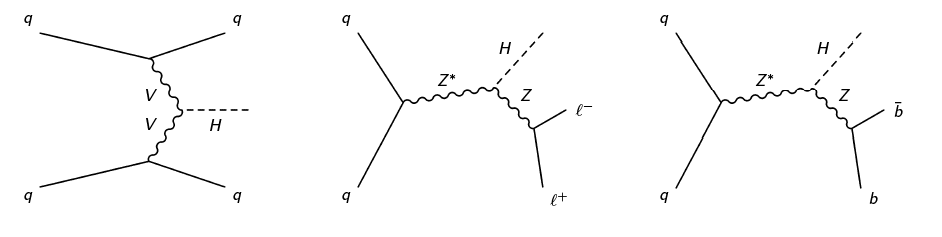
\includegraphics[width=\textwidth]{TalkPics/invcomb021213/feyndiags}
  %% \begin{fmfgraph*}(100,70)
  %%         \fmfleft{i1,i2}
  %%         \fmfright{o1,o2,o3}
  %%         \fmf{fermion}{i1,v1,o1}
  %%         \fmf{fermion}{i2,v2,o3}
  %%         \fmf{phantom,tension=4/5}{v1,v2}
  %%         \fmffreeze
  %%         \fmf{photon,label=$W,,Z$}{v1,v3}
  %%         \fmf{photon,label=$W,,Z$}{v2,v3}
  %%         \fmf{dashes}{v3,o2}
  %%         \fmflabel{$q$}{i1}
  %%         \fmflabel{$q$}{i2}
  %%         \fmflabel{$q$}{o1}
  %%         \fmflabel{$q$}{o3}
  %%         \fmflabel{$H$}{o2}
  %%       \end{fmfgraph*}
}
\date{}
\begin{document}
\begin{fmffile}{higgsexoupdatefeyndiags}
\tikzstyle{every picture}+=[remember picture]

%TITLE PAGE
\section{Title}
\begin{frame}
  \titlepage
  
\end{frame}

\begin{frame}
  \frametitle{W MC Reminder}
  \begin{block}{}
    \begin{itemize}
    \item Control plots shown last week
    \item Significant differences seen in shape between run 1 and run 2
    \item[-] Possible bias from Met Significance differences
    \end{itemize}
    \end{block}
\end{frame}

\begin{frame}
  \frametitle{Closer W Comparison}
  \begin{block}{}
    \begin{itemize}
    \item Run 1 Met significance variable recalculated from light trees:
    \item[-] $\frac{MET}{\sqrt{\Sigma E_T}}>3.0$
    \item Distributions still normalised to 1
    \item Selection as loose as possible: $\eta_{j1} \cdot \eta_{j2}<0,\, \eta_{j1}<4.7,\, \eta_{j2}<4.7,$
      $p_{T}^{\text{j1}}>30 \,\text{GeV},\,p_{T}^{\text{j2}}>30\,\text{GeV},$
      $\Delta\eta_{jj}>3.6,METsig>3.$
    \item Only munu shown
    \end{itemize}
  \end{block}
\end{frame}

\begin{frame}
  \frametitle{W munu Comparison: run 1 vs run 2: Jet $p_{T}$}
  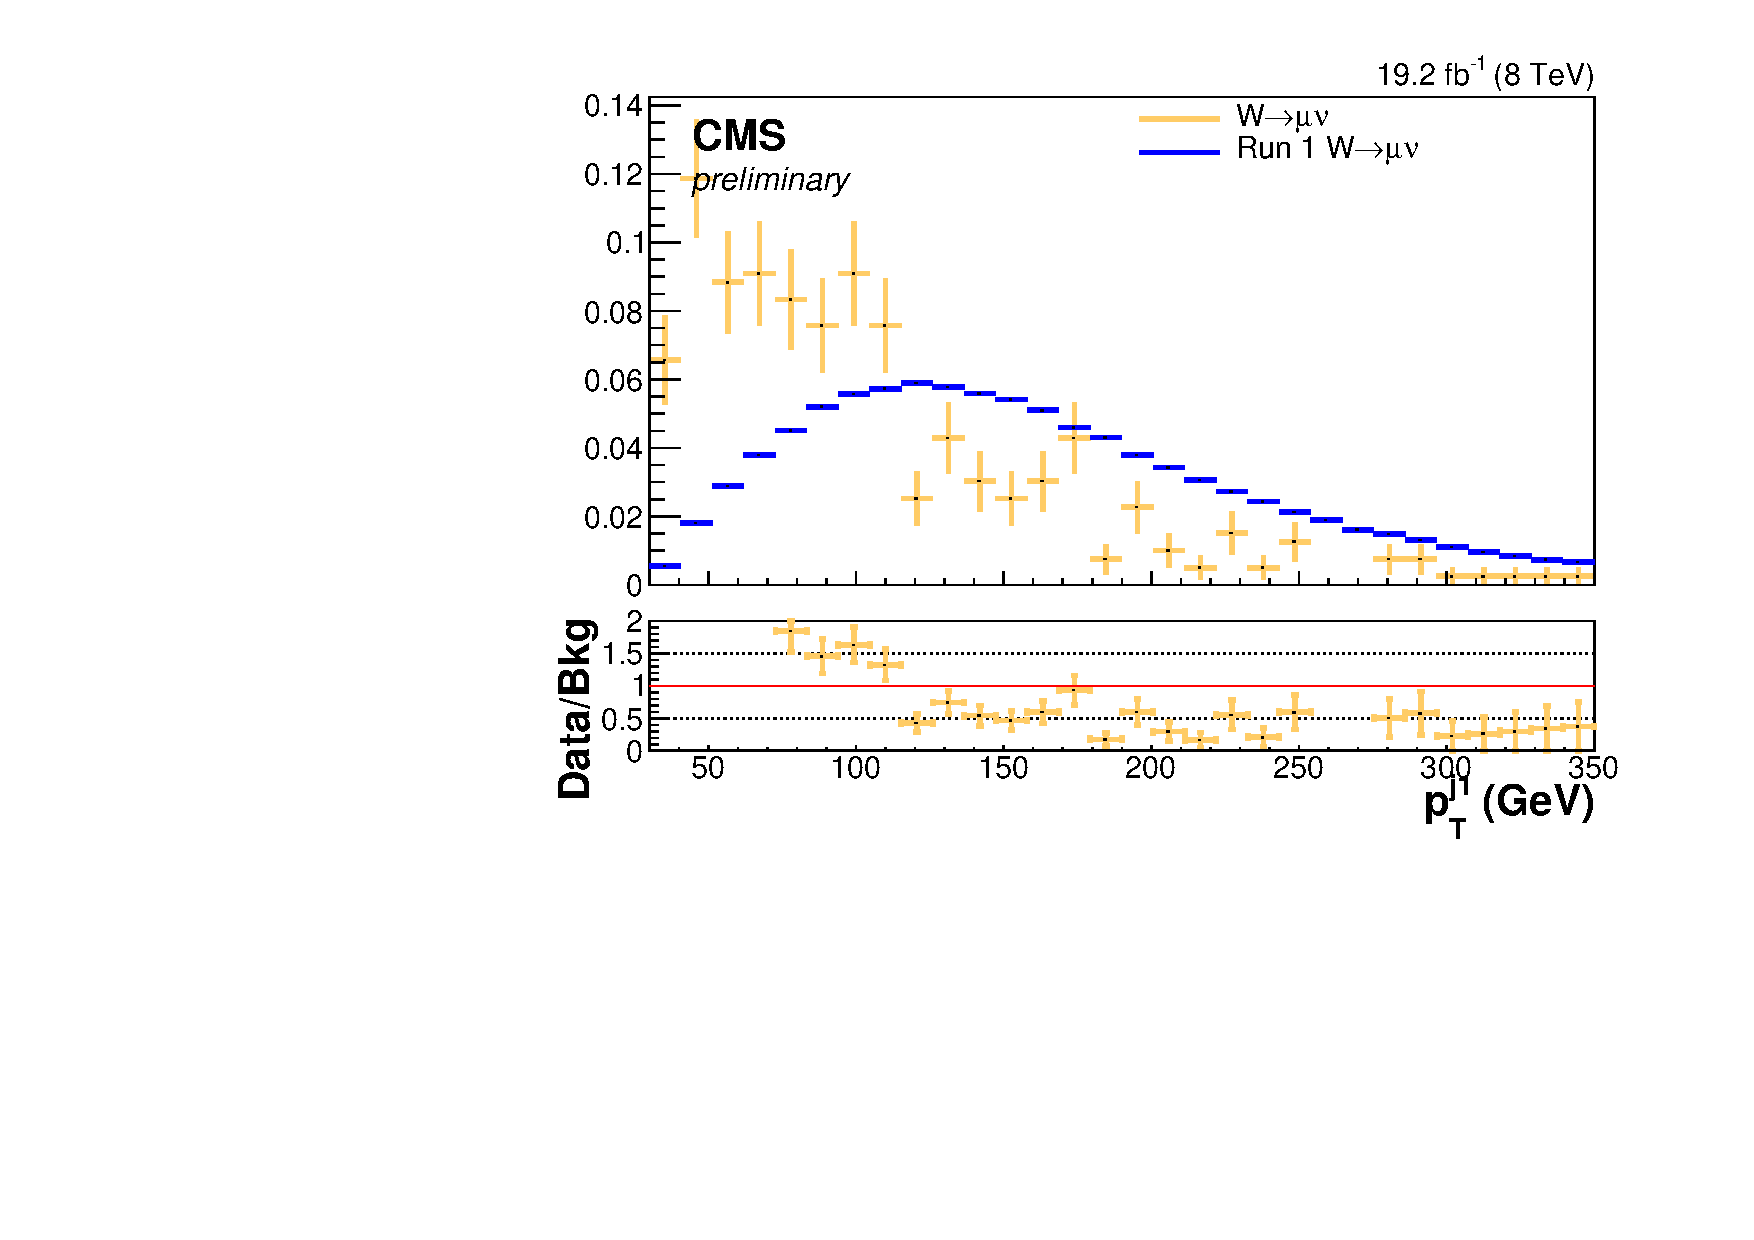
\includegraphics[width=.5\textwidth]{TalkPics/geninfo220615/output_run1comparegen220615/munu_norm_jet1_pt.pdf}
  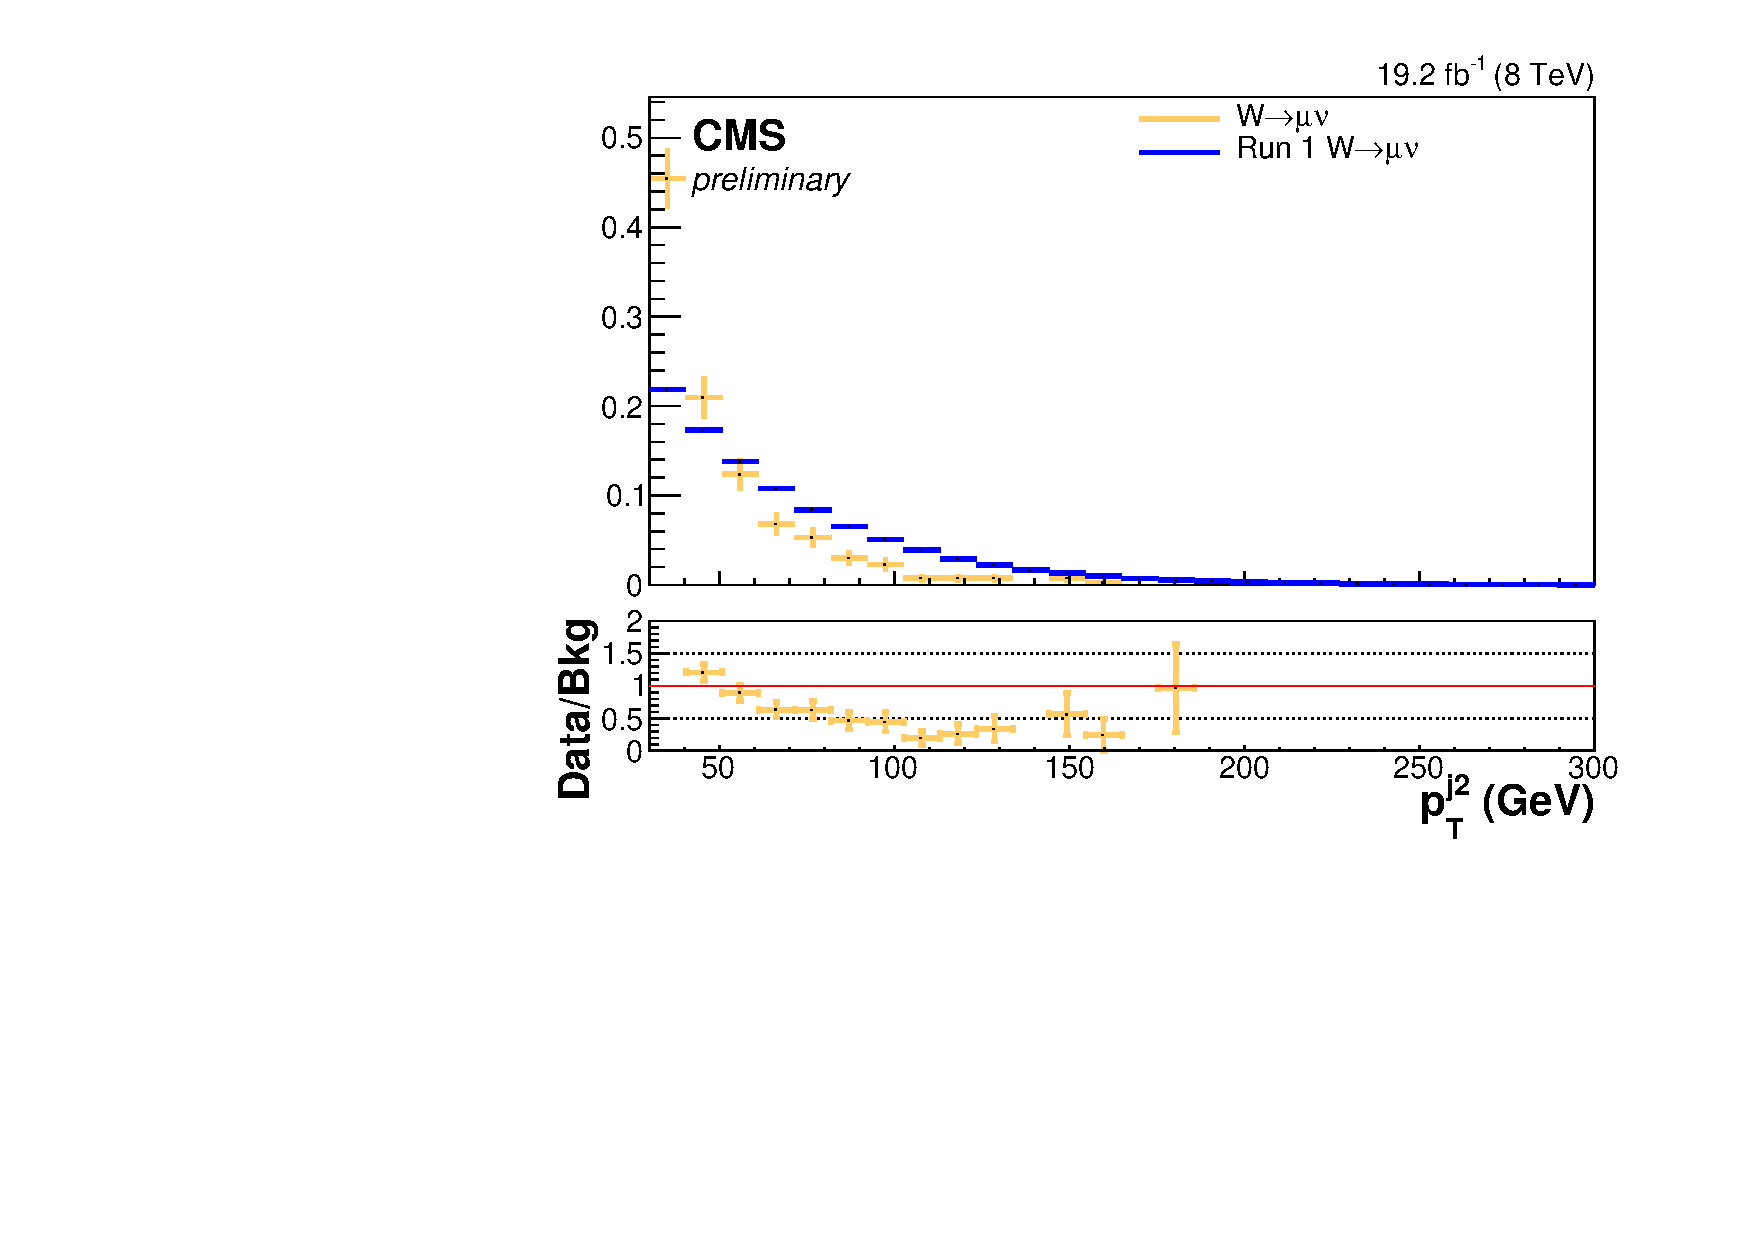
\includegraphics[width=.5\textwidth]{TalkPics/geninfo220615/output_run1comparegen220615/munu_norm_jet2_pt.pdf}
  \begin{block}{}
    \begin{itemize}
    \item Agreement better but still significant differences
    \item[-] Especially for low values
    \end{itemize}
  \end{block}
\end{frame}

\begin{frame}
  \frametitle{W munu Comparison: run 1 vs run 2: Jet $\eta$}
  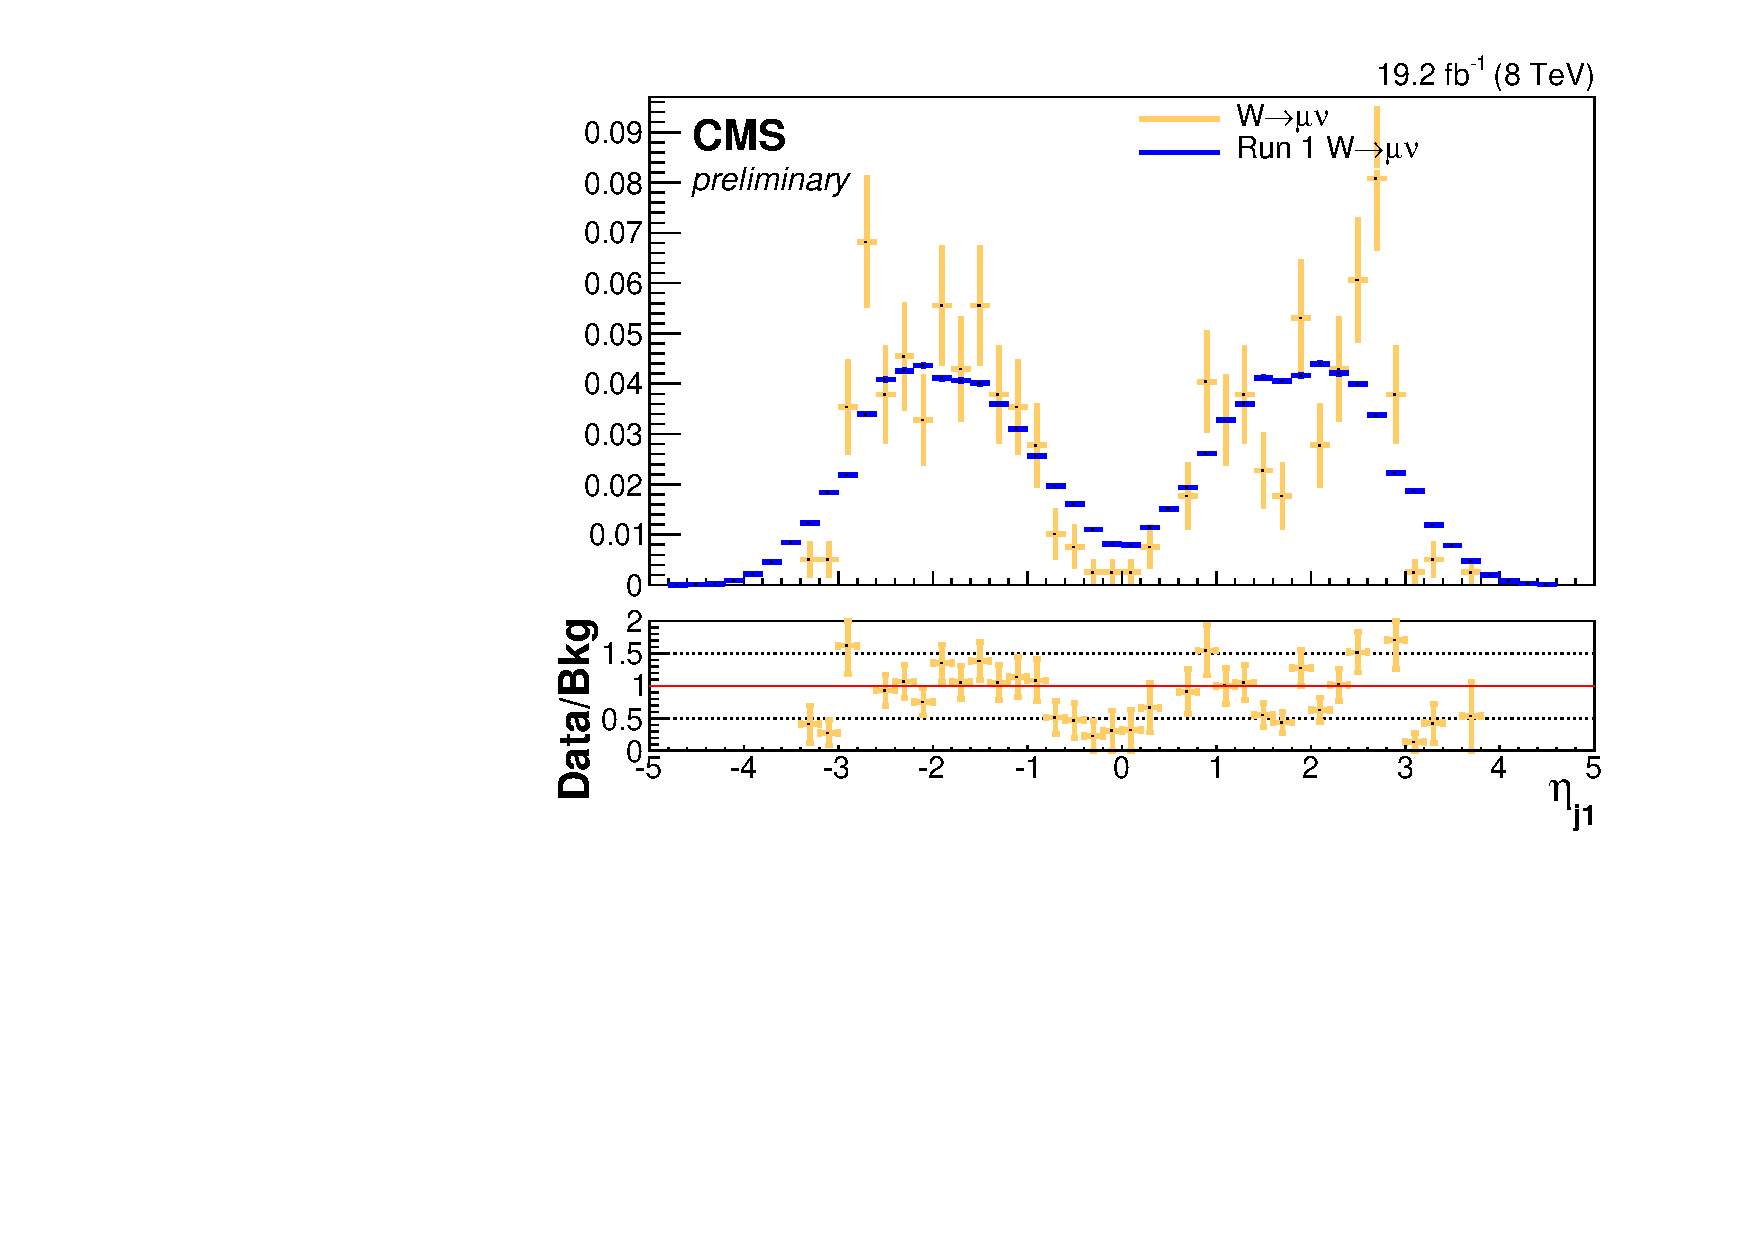
\includegraphics[width=.5\textwidth]{TalkPics/geninfo220615/output_run1comparegen220615/munu_norm_jet1_eta.pdf}
  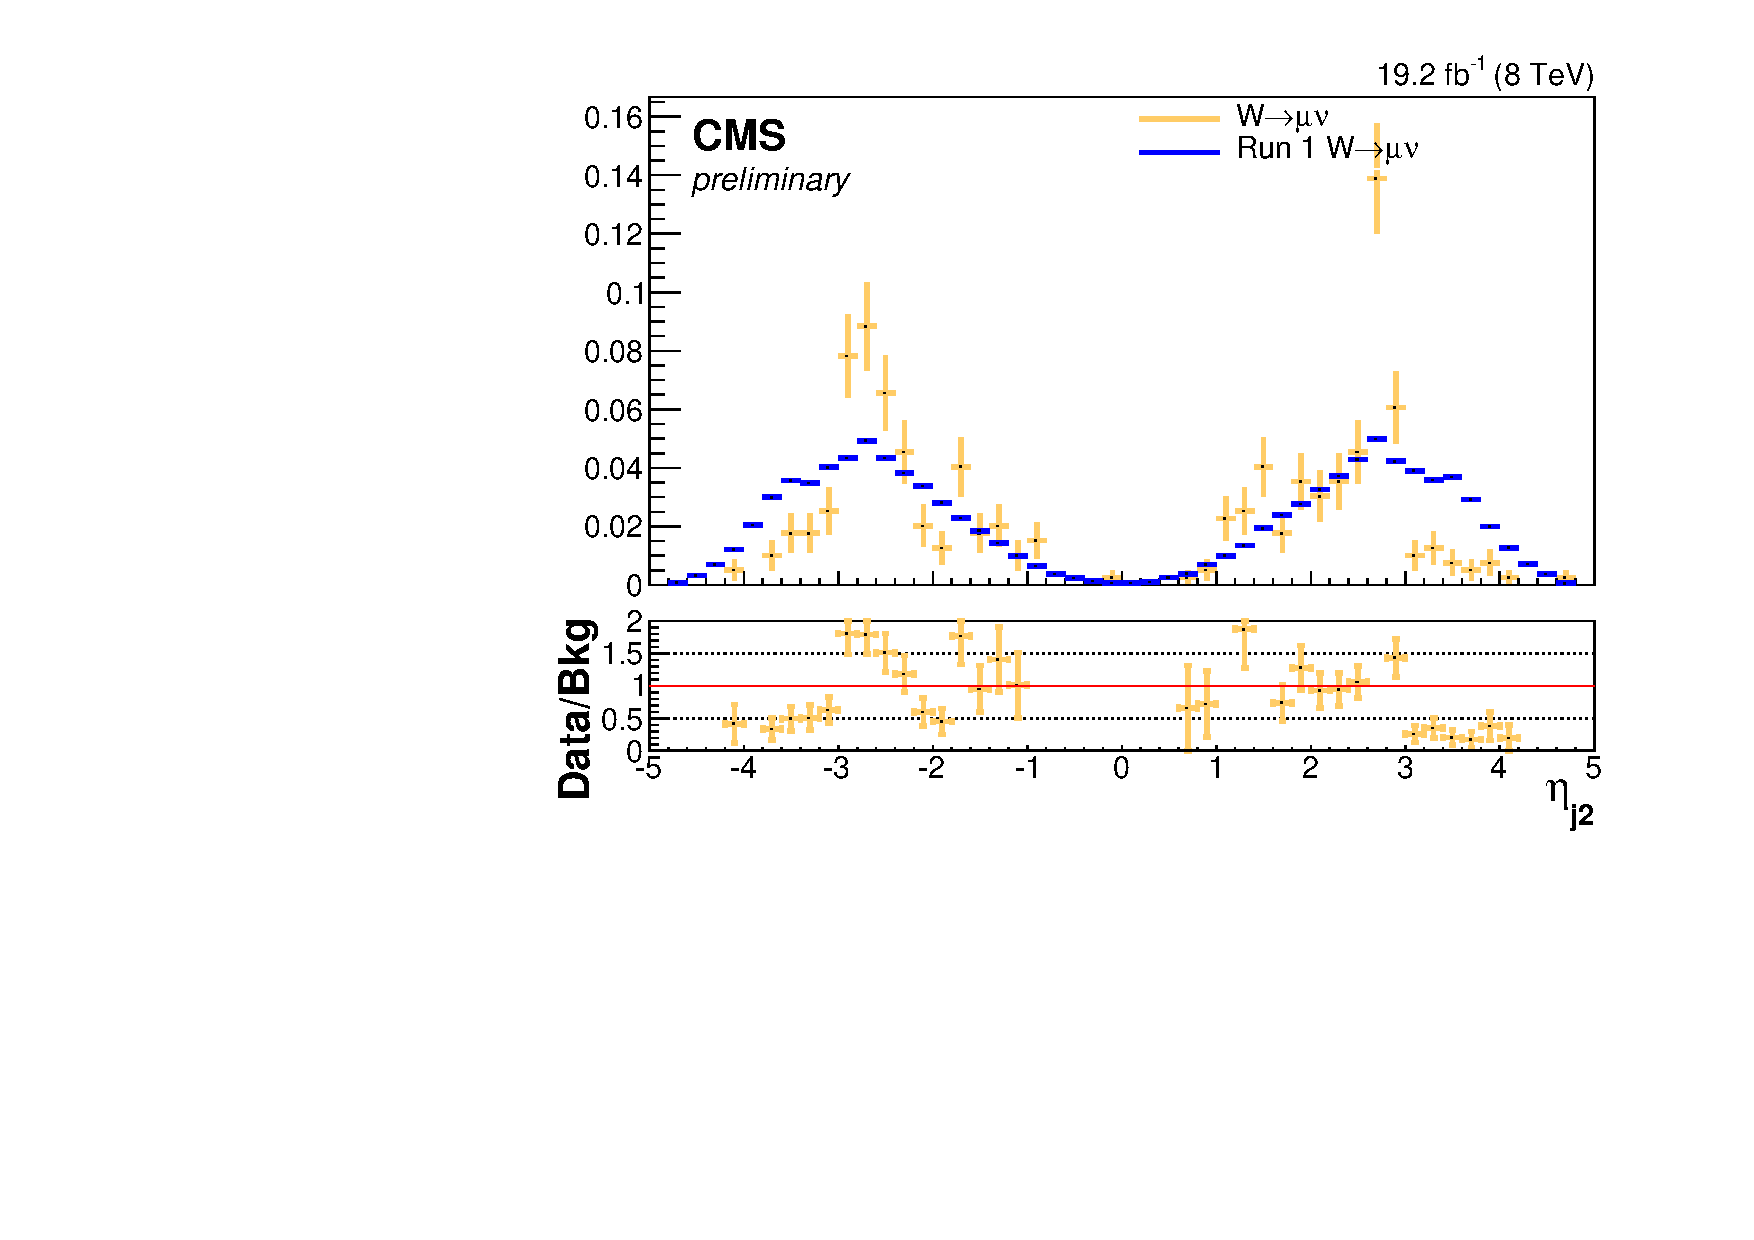
\includegraphics[width=.5\textwidth]{TalkPics/geninfo220615/output_run1comparegen220615/munu_norm_jet2_eta.pdf}
\end{frame}

\begin{frame}
  \frametitle{W munu Comparison: run 1 vs run 2: Jet $\phi$}
  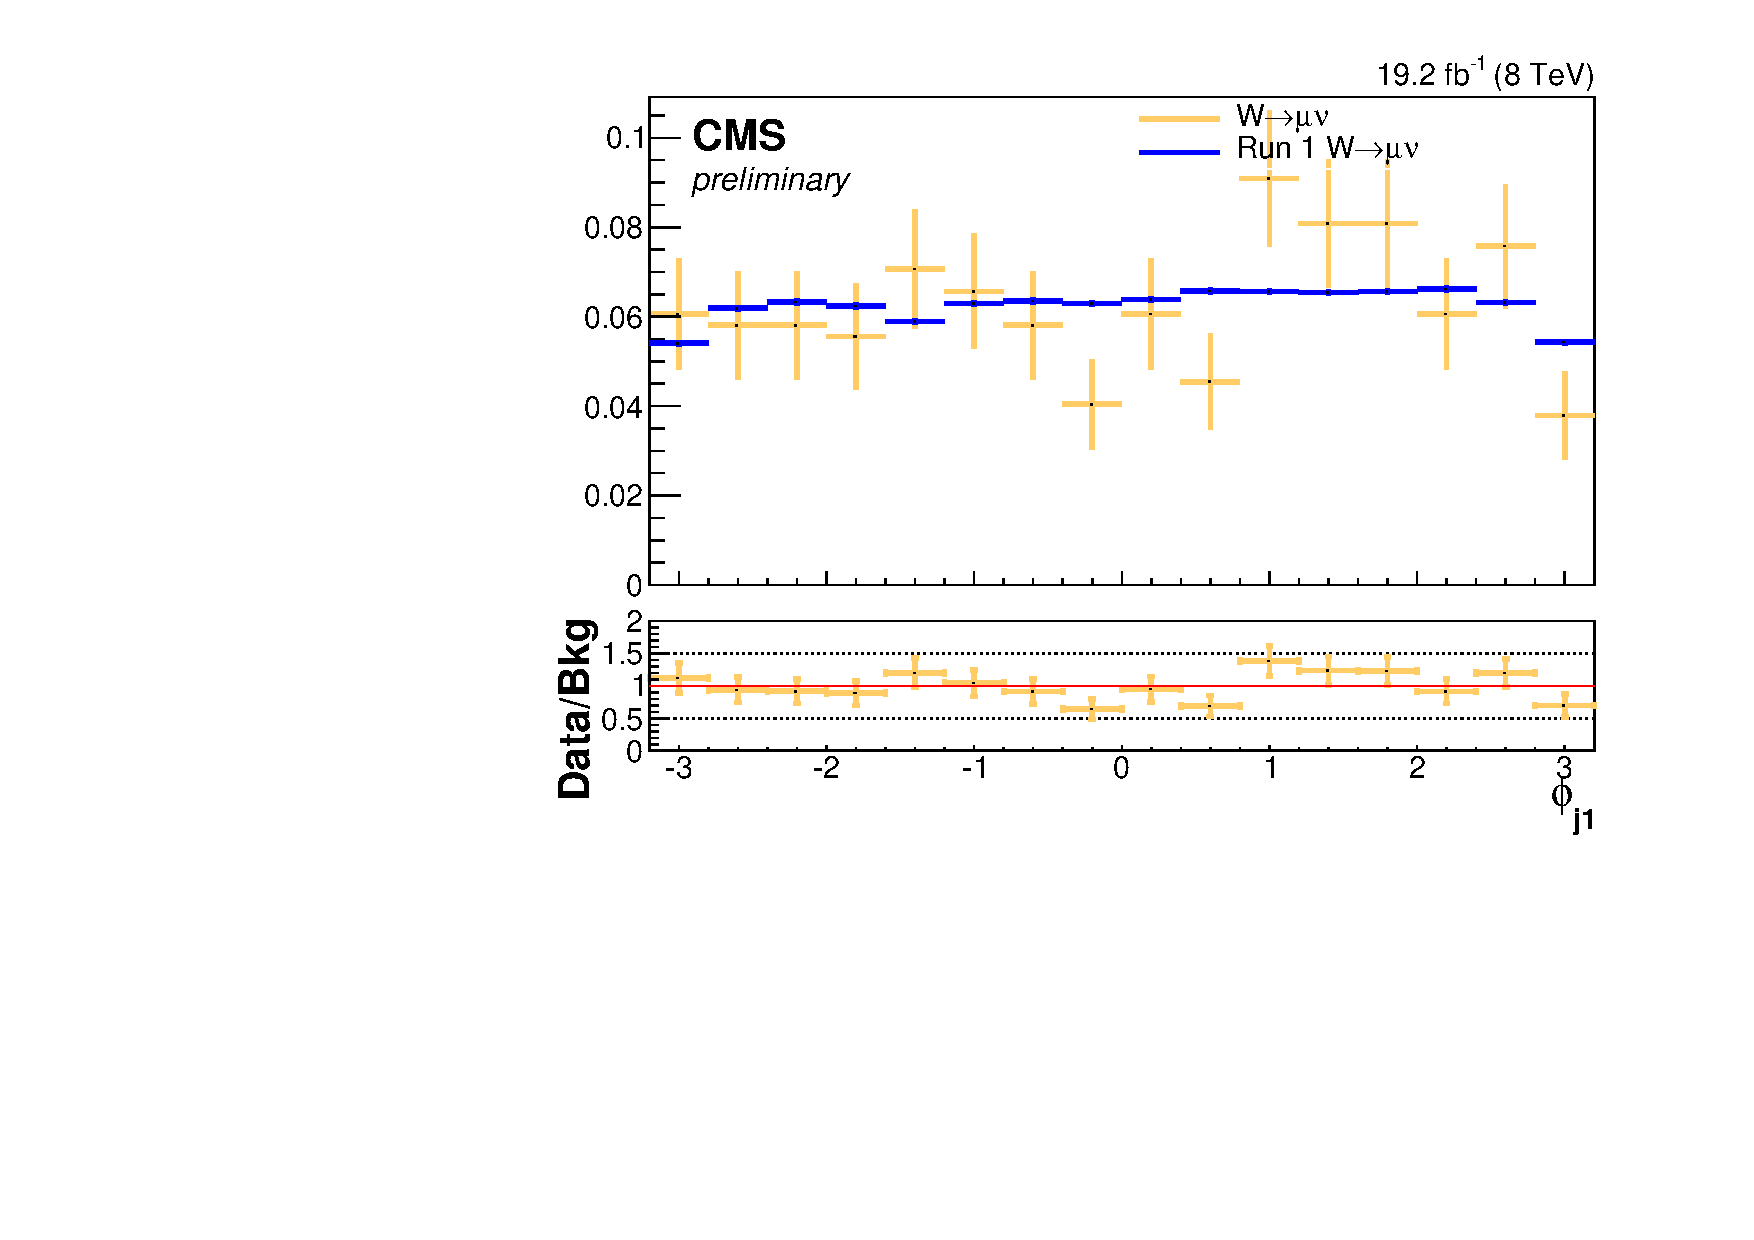
\includegraphics[width=.5\textwidth]{TalkPics/geninfo220615/output_run1comparegen220615/munu_norm_jet1_phi.pdf}
  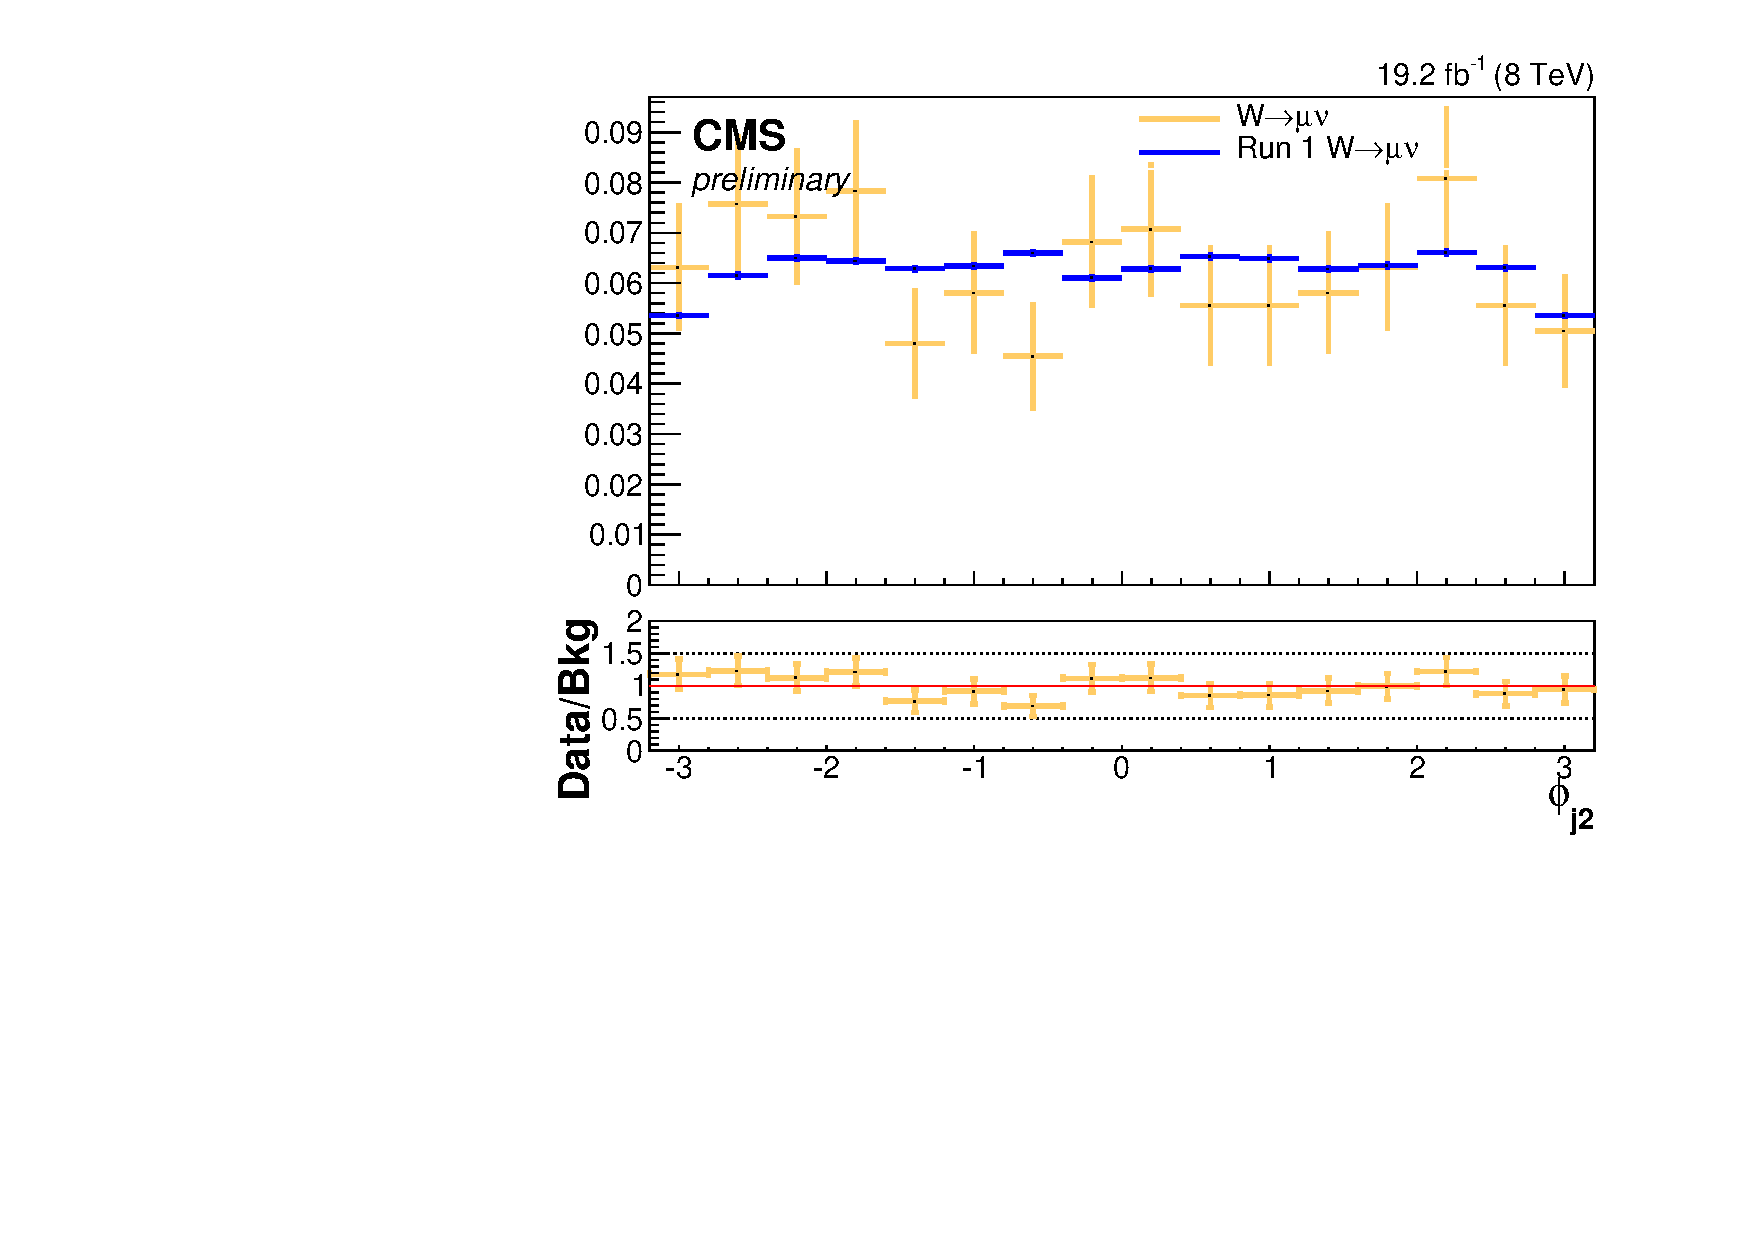
\includegraphics[width=.5\textwidth]{TalkPics/geninfo220615/output_run1comparegen220615/munu_norm_jet2_phi.pdf}
  \begin{block}{}
    \begin{itemize}
    \item $\phi$ distributions look similar within stat error
    \end{itemize}
  \end{block}
\end{frame}

\begin{frame}
  \frametitle{W munu Comparison: run 1 vs run 2: Met}
  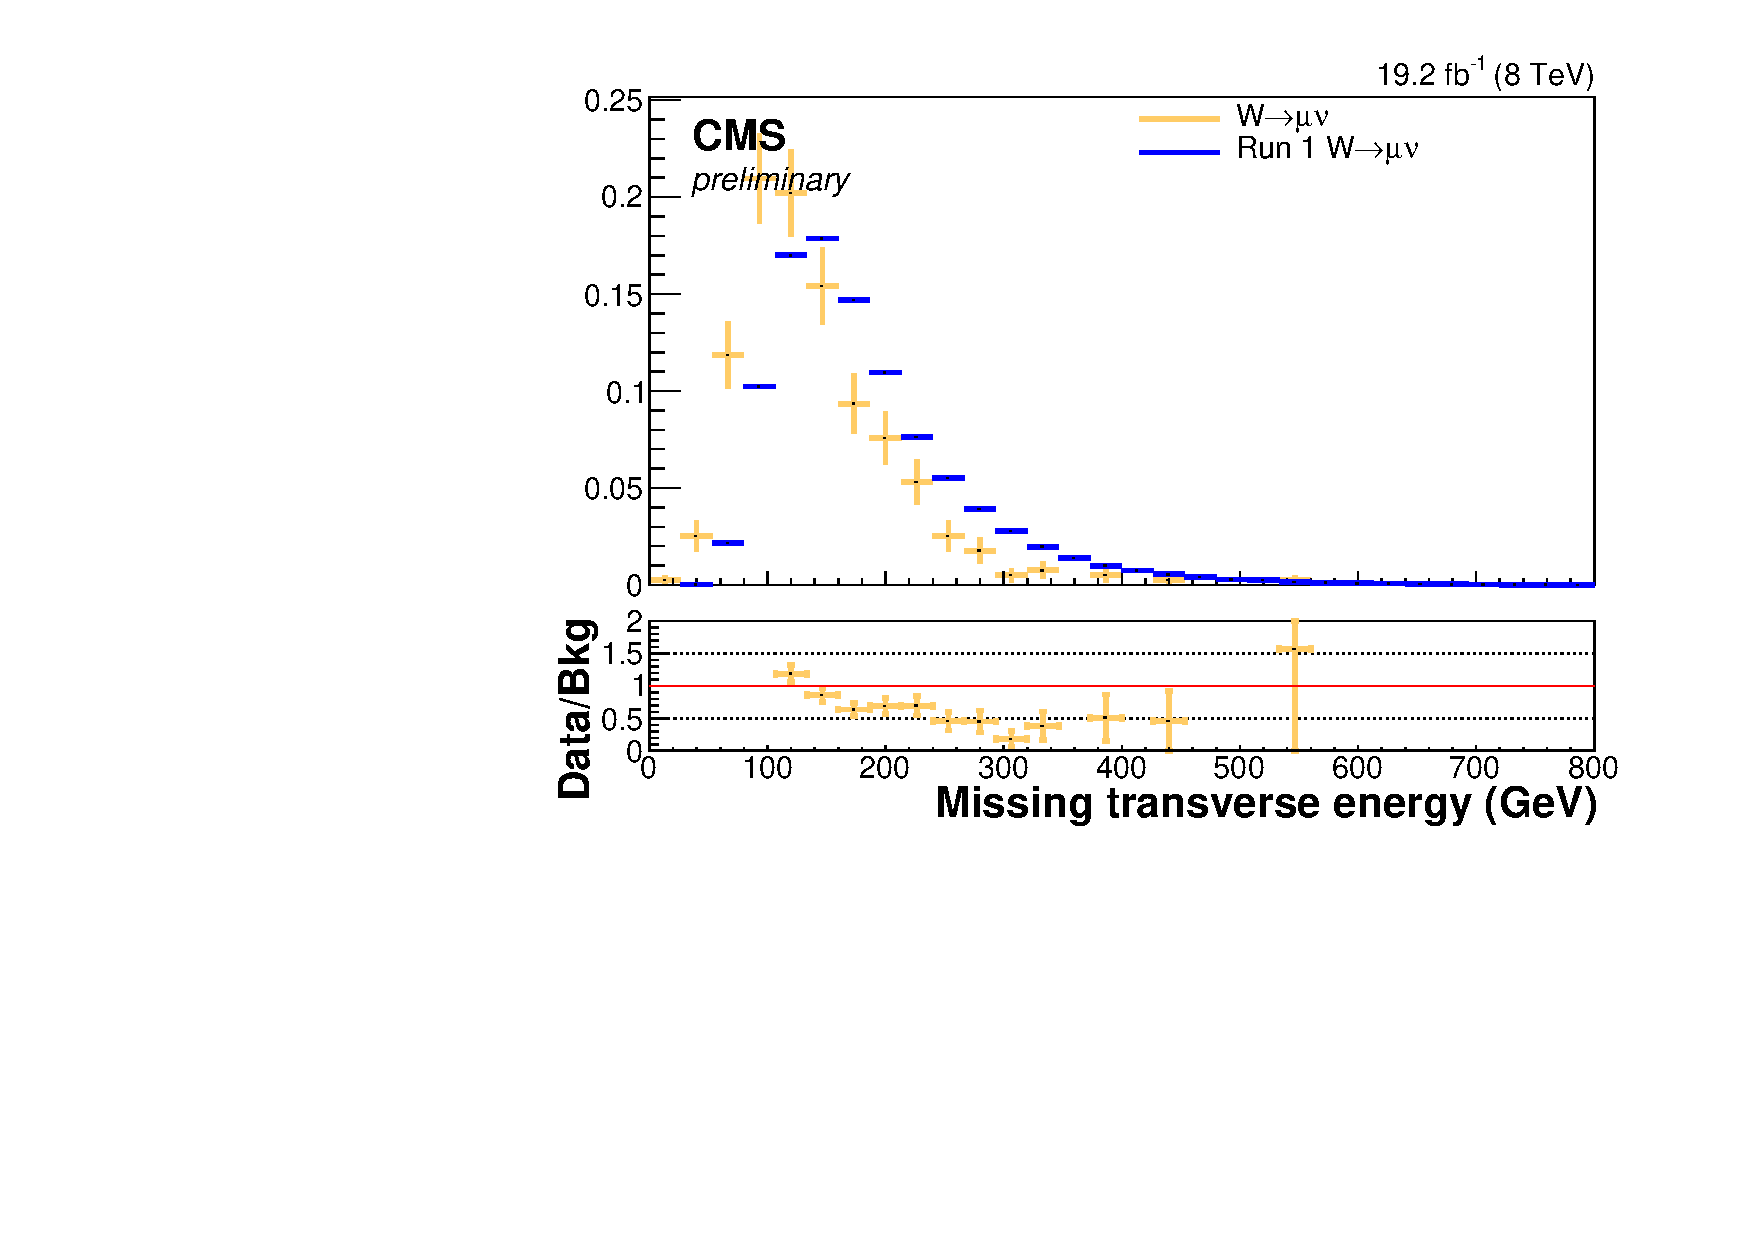
\includegraphics[width=.5\textwidth]{TalkPics/geninfo220615/output_run1comparegen220615/munu_norm_metnomuons.pdf}
  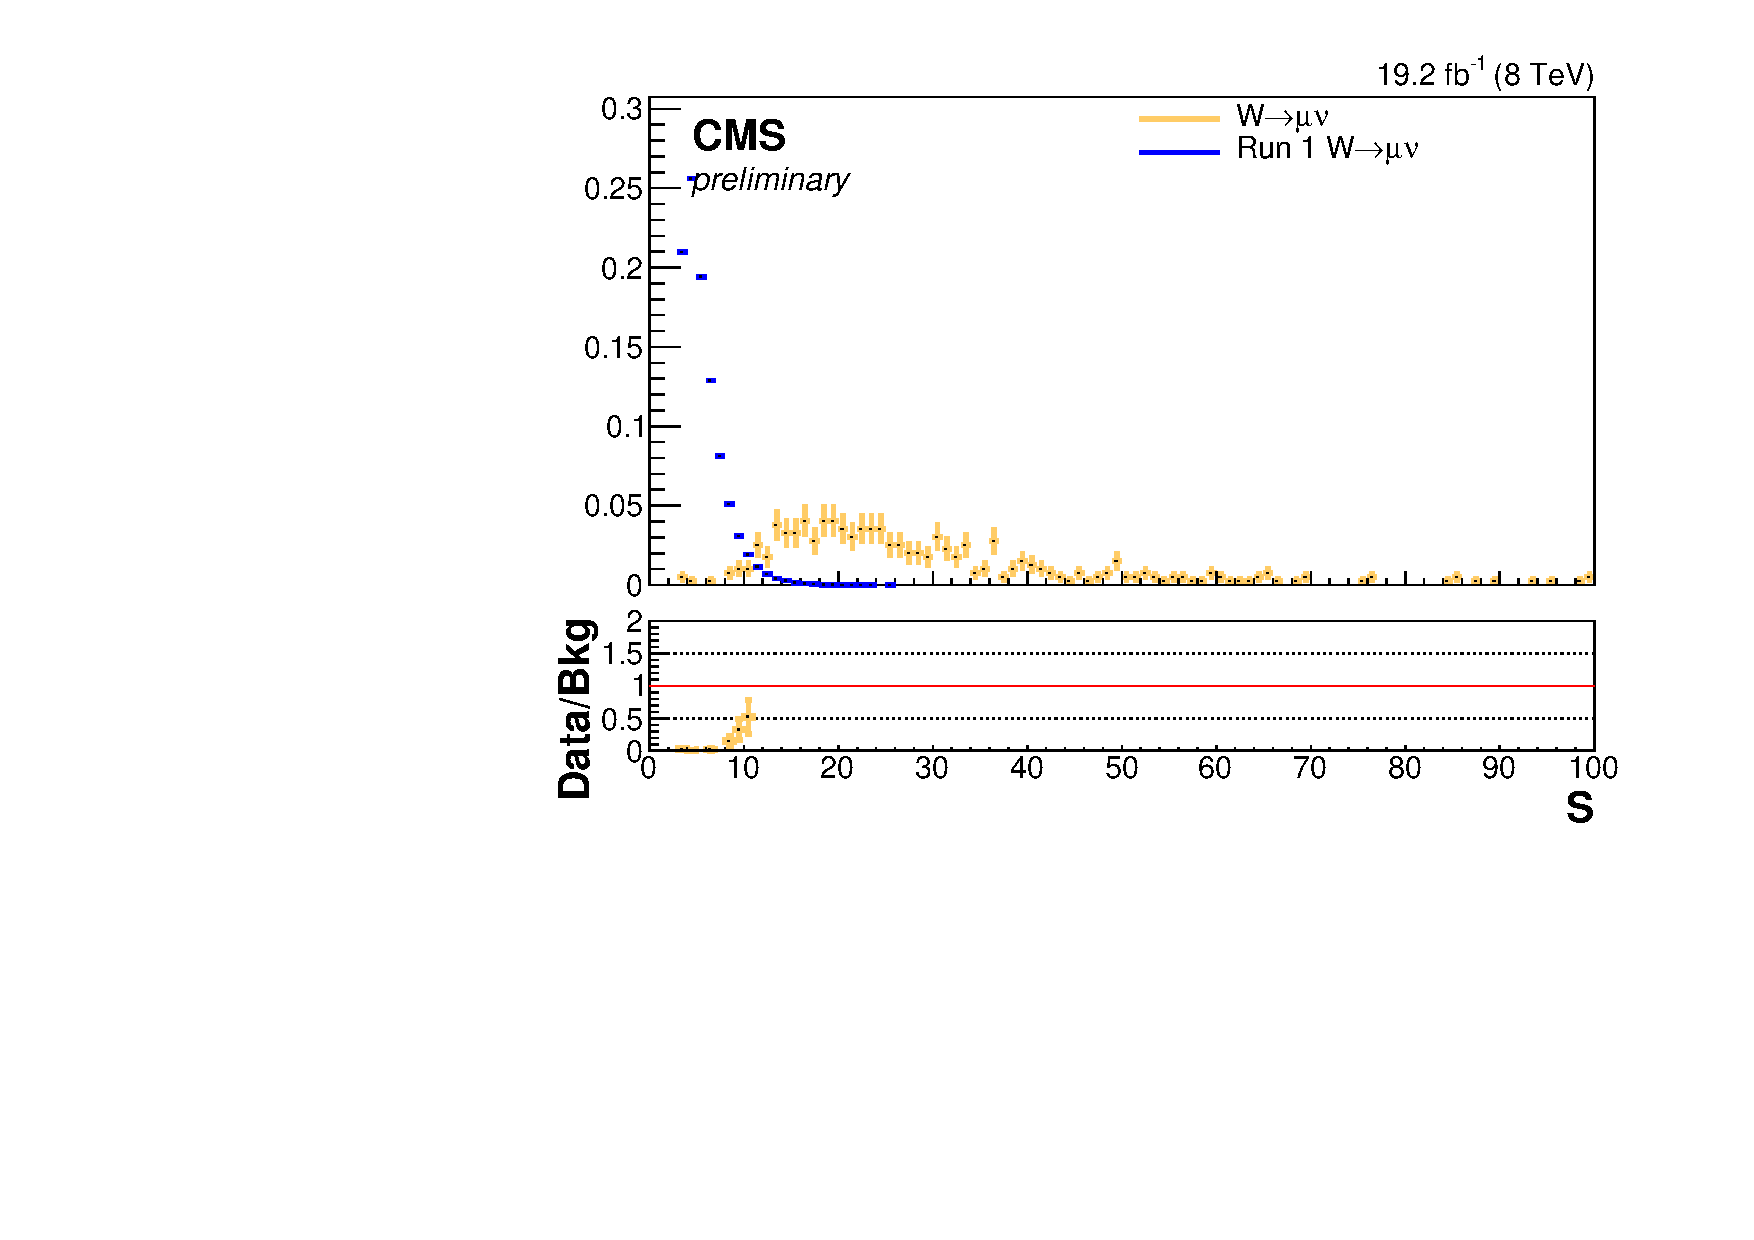
\includegraphics[width=.5\textwidth]{TalkPics/geninfo220615/output_run1comparegen220615/munu_norm_metnomu_significance.pdf}
  \begin{block}{}
    \begin{itemize}
    \item Metnomu more similar
    \item Met significance variable difference now apparent
    \end{itemize}
  \end{block}
\end{frame}

\begin{frame}
  \frametitle{W munu Comparison: run 1 vs run 2: $\Delta\phi$ variables}
  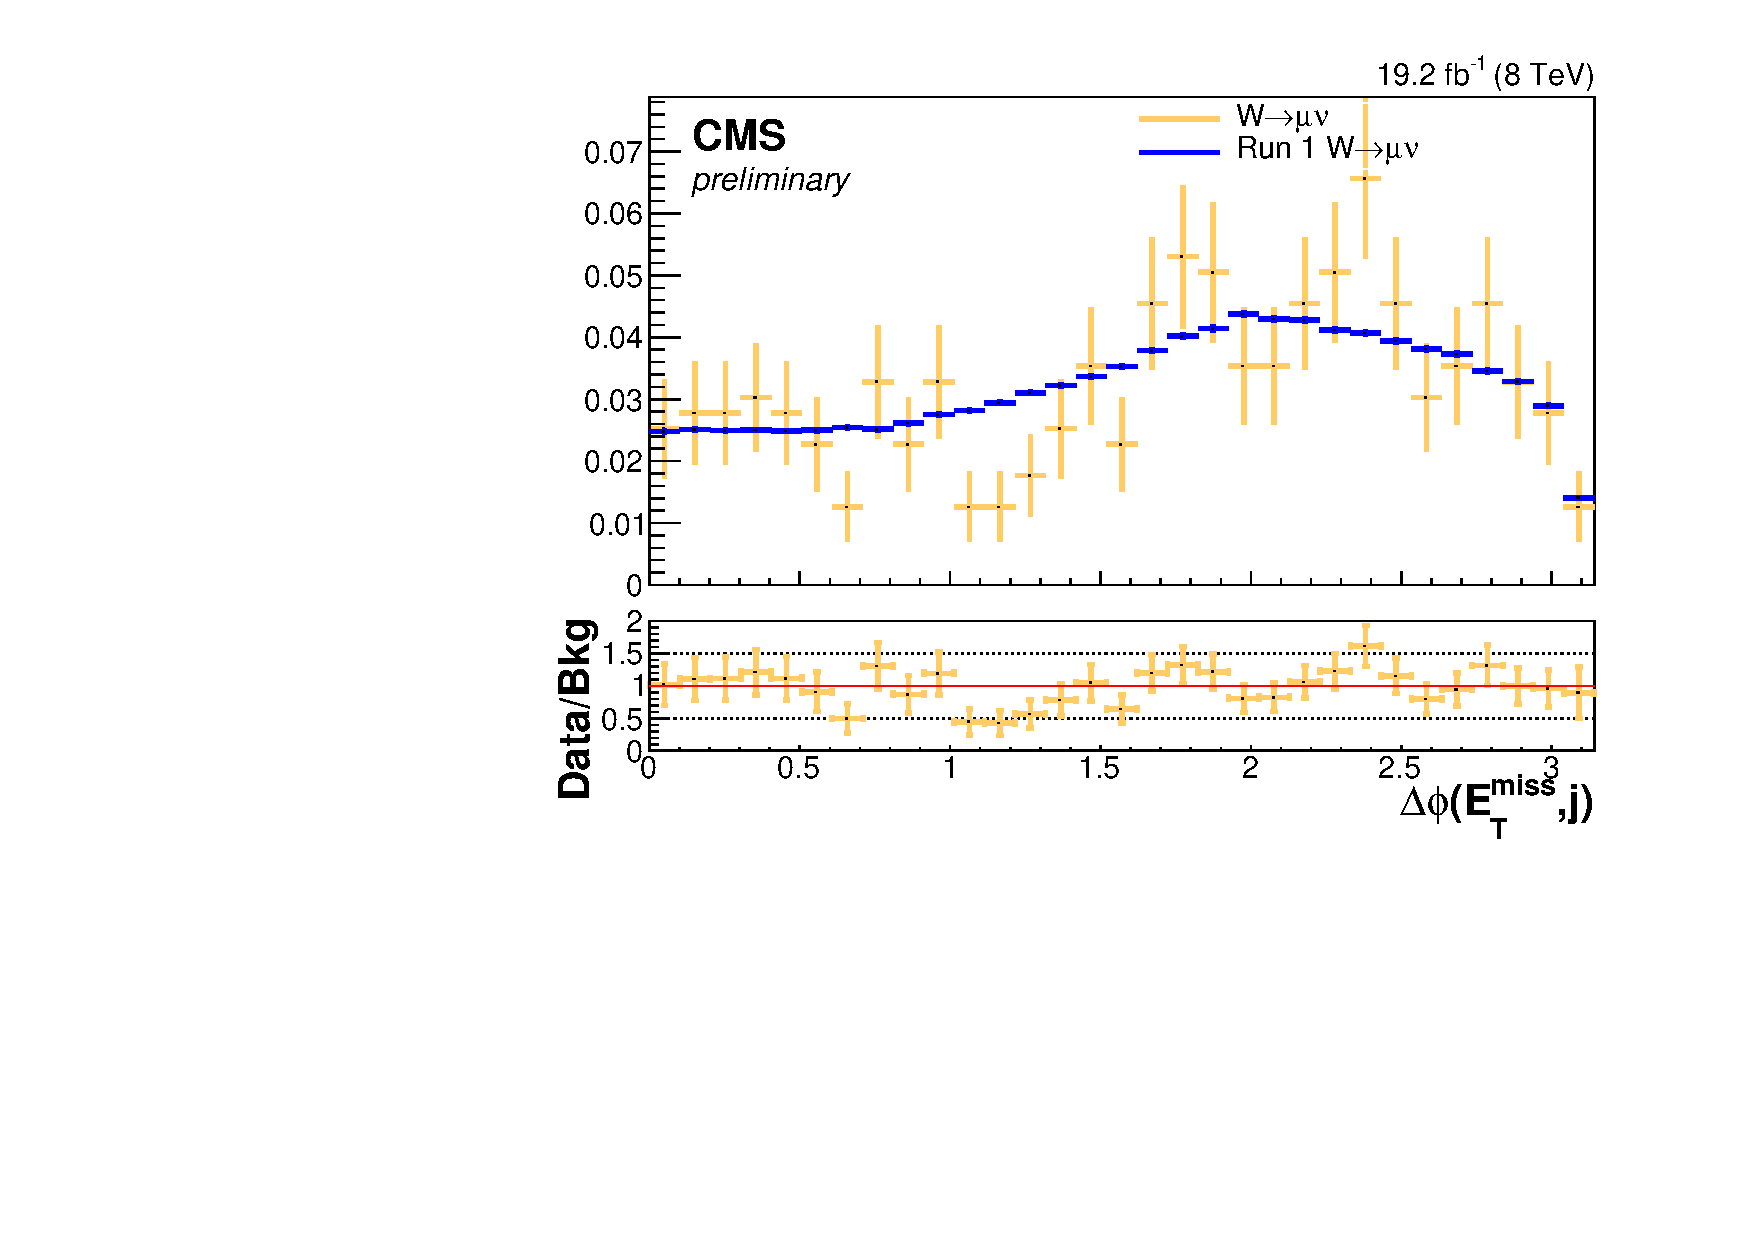
\includegraphics[width=.5\textwidth]{TalkPics/geninfo220615/output_run1comparegen220615/munu_norm_alljetsmetnomu_mindphi.pdf}
  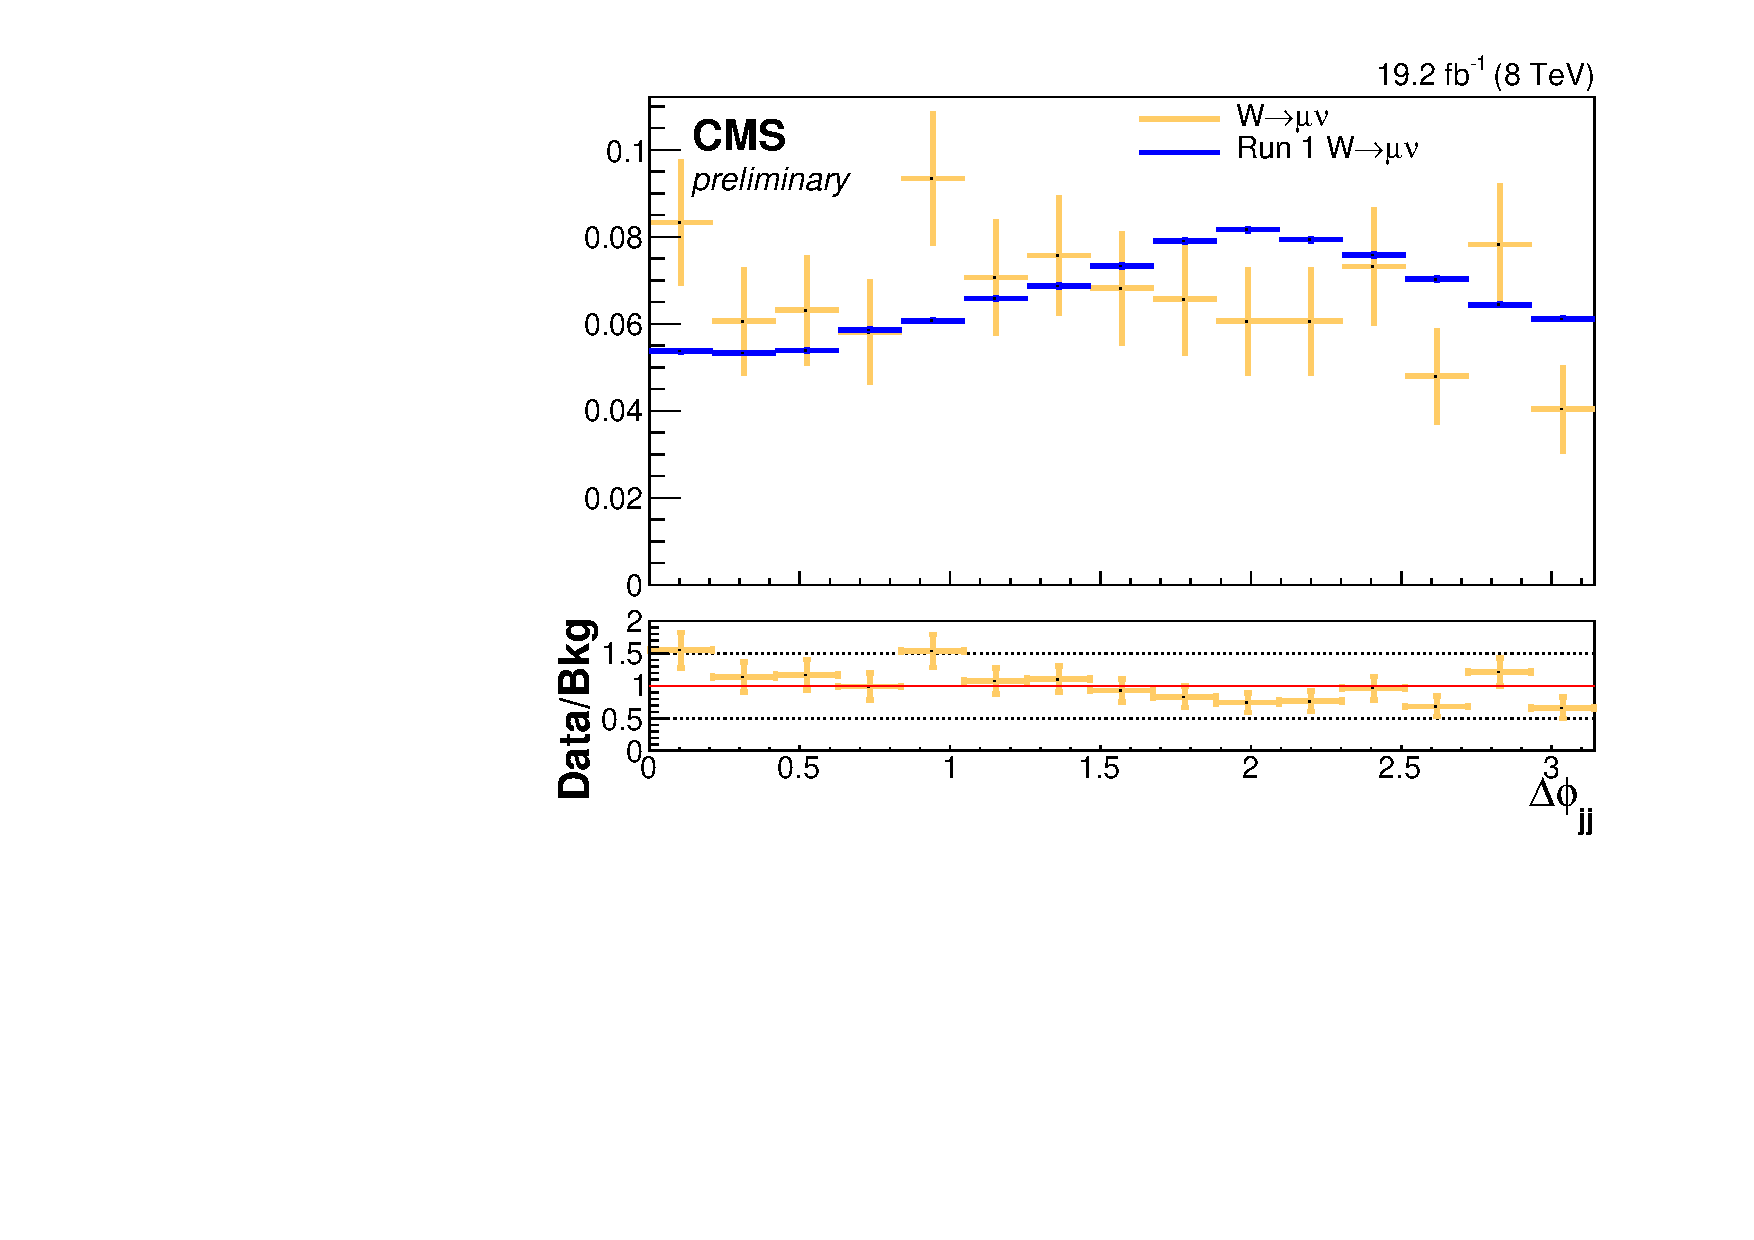
\includegraphics[width=.5\textwidth]{TalkPics/geninfo220615/output_run1comparegen220615/munu_norm_dijet_dphi.pdf}
  \begin{block}{}
    \begin{itemize}
    \item Much more similar than last week
    \end{itemize}
  \end{block}
\end{frame}

\begin{frame}
  \frametitle{W munu Comparison: run 1 vs run 2: dijet variables}
  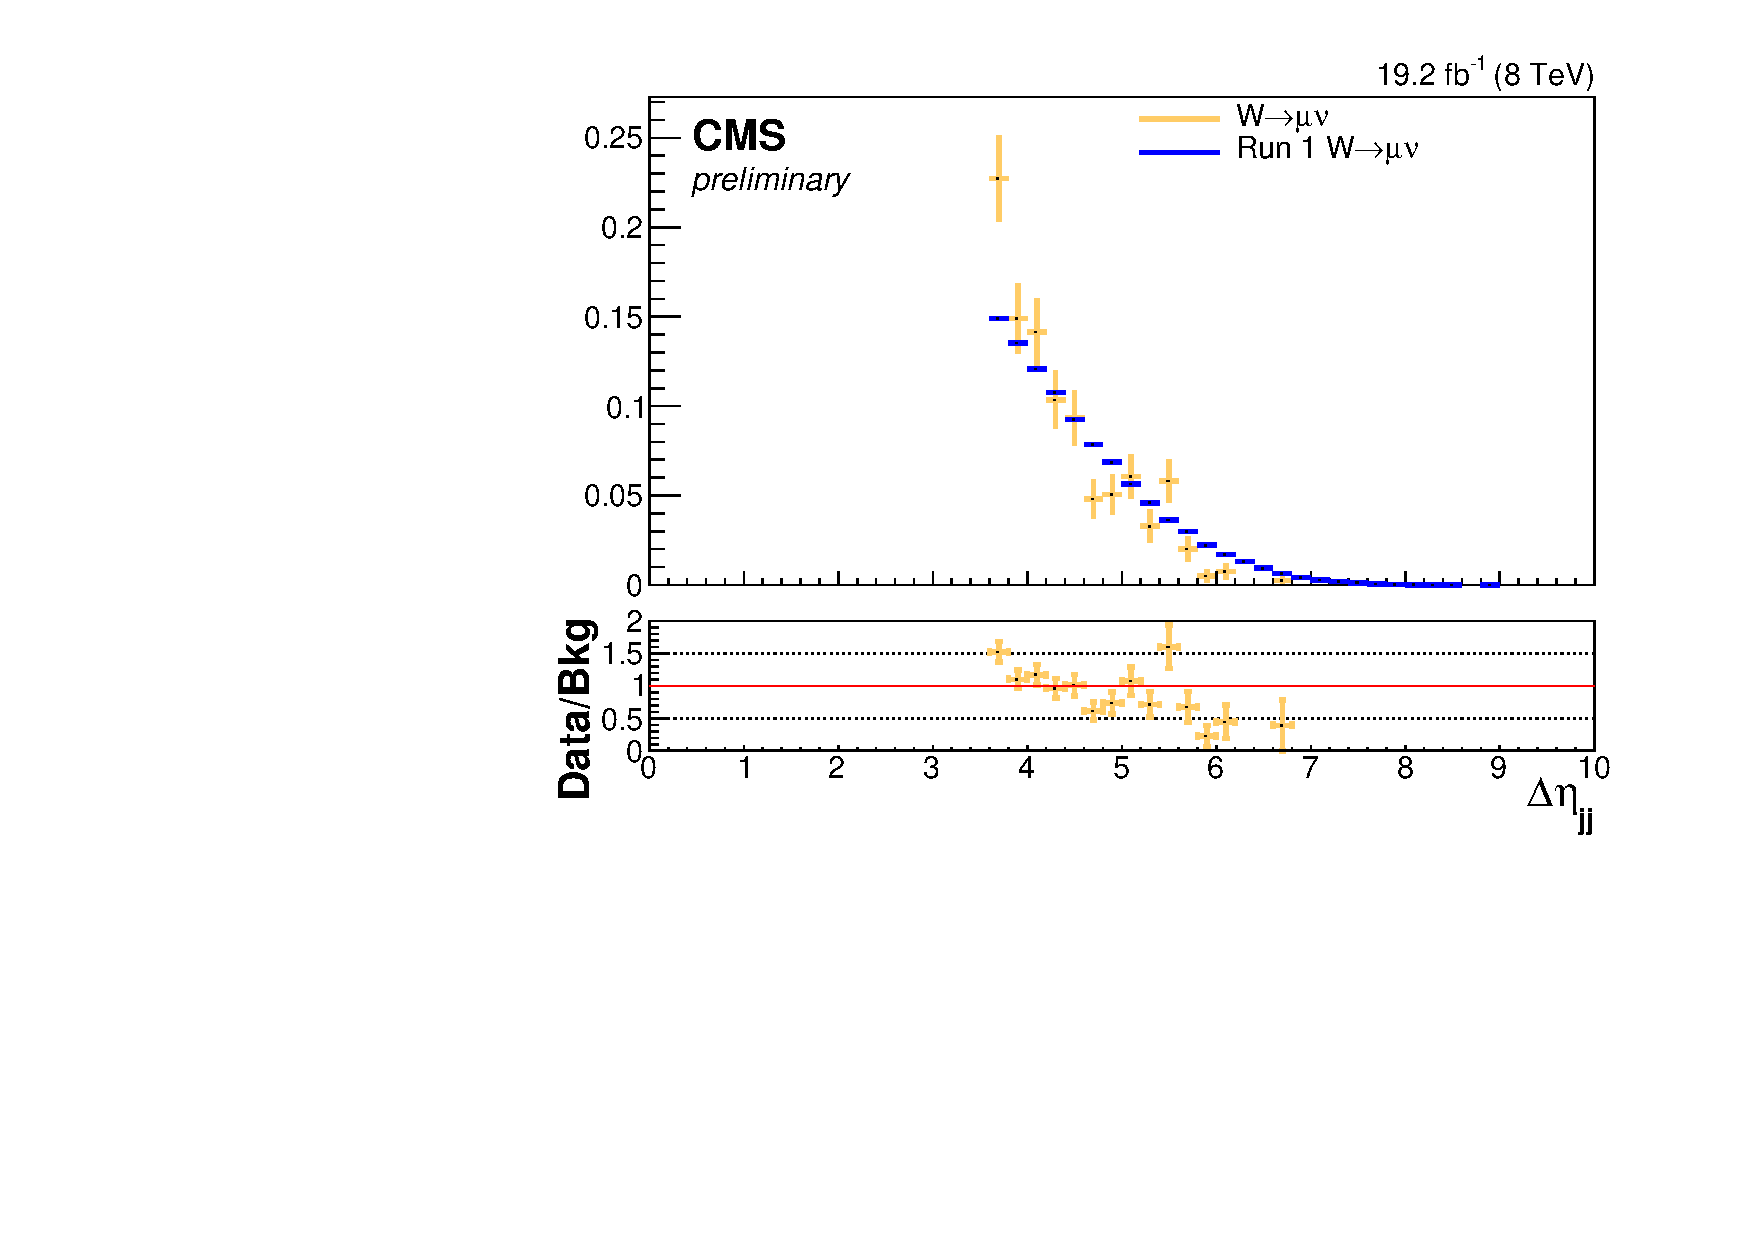
\includegraphics[width=.5\textwidth]{TalkPics/geninfo220615/output_run1comparegen220615/munu_norm_dijet_deta.pdf}
  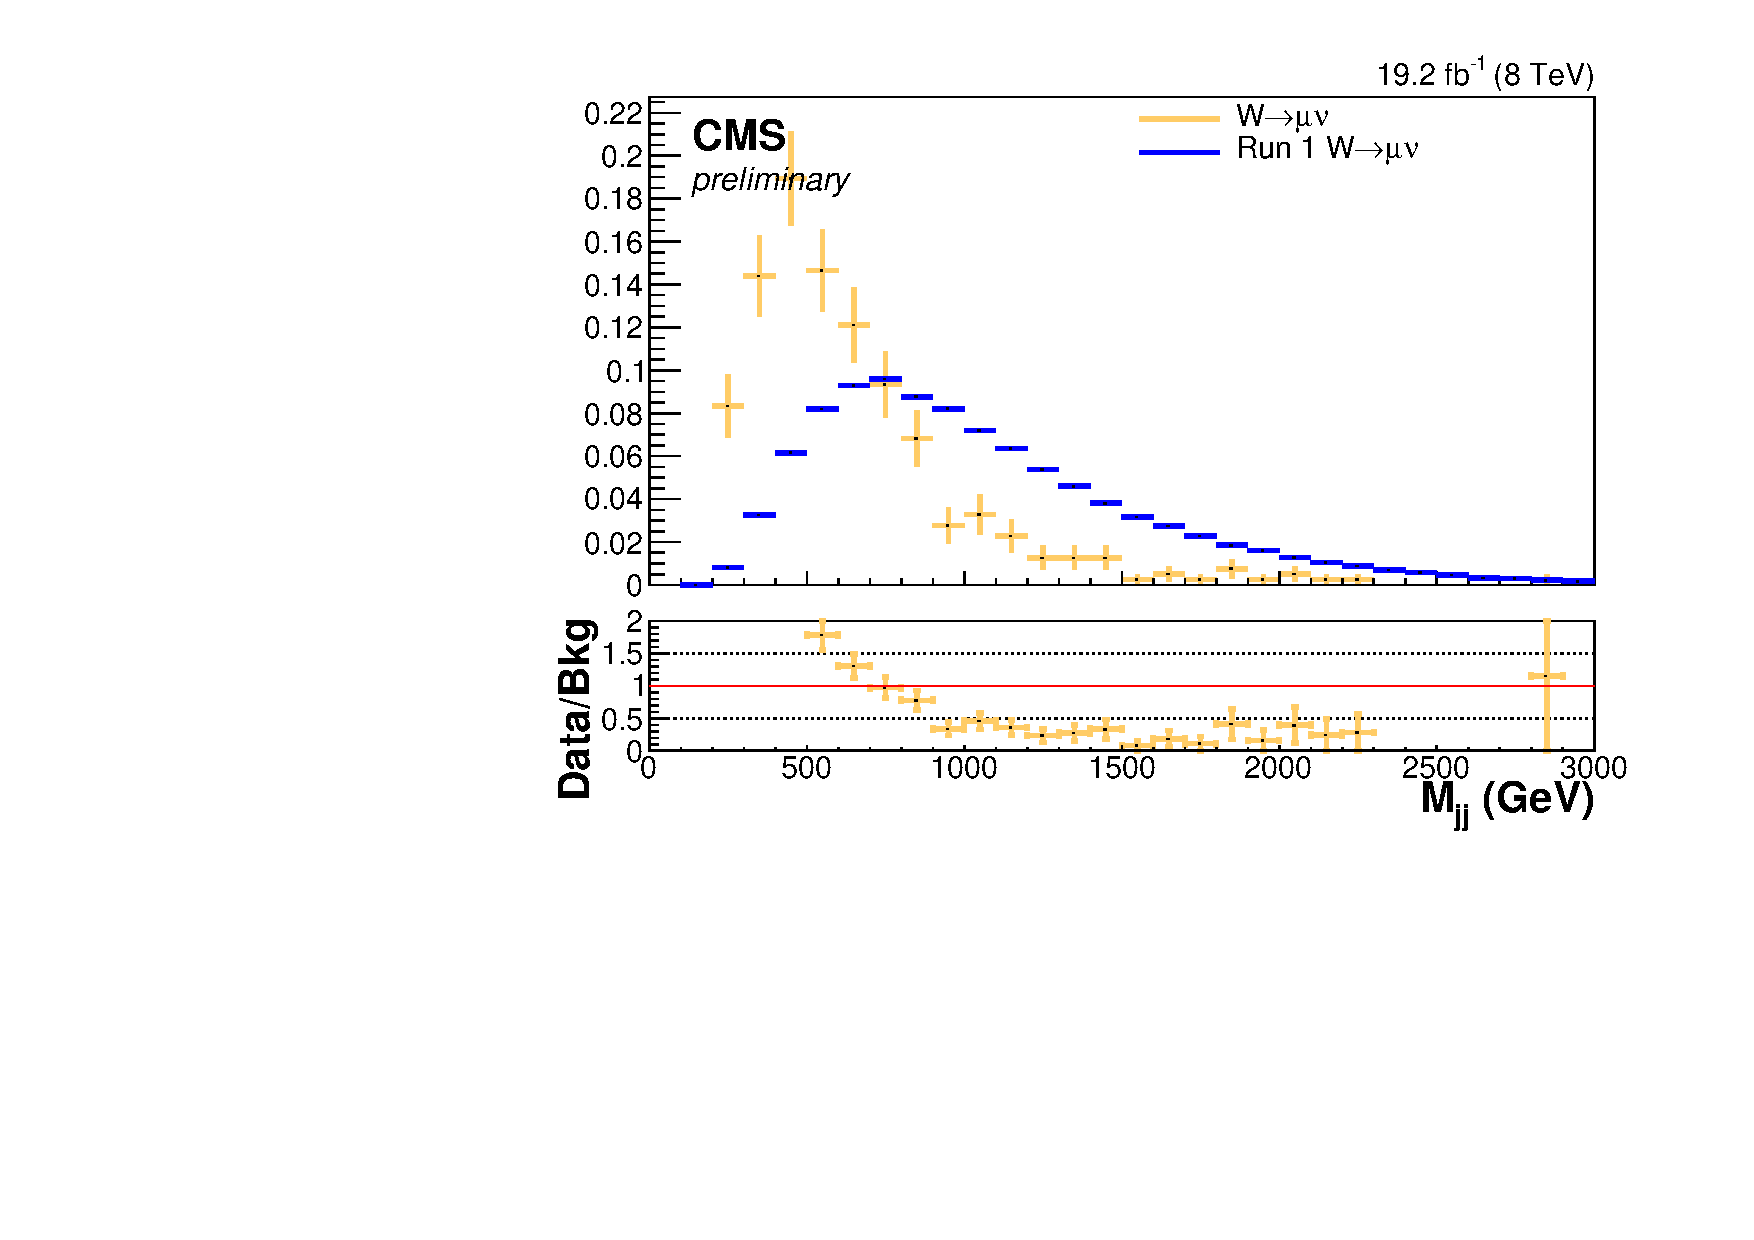
\includegraphics[width=.5\textwidth]{TalkPics/geninfo220615/output_run1comparegen220615/munu_norm_dijet_M.pdf}
  \begin{block}{}
    \begin{itemize}
    \item Mjj distribution very different up to 800 GeV then similar
    \end{itemize}
  \end{block}
\end{frame}

\begin{frame}
  \frametitle{W munu Comparison: run 1 vs run 2: N jets}
  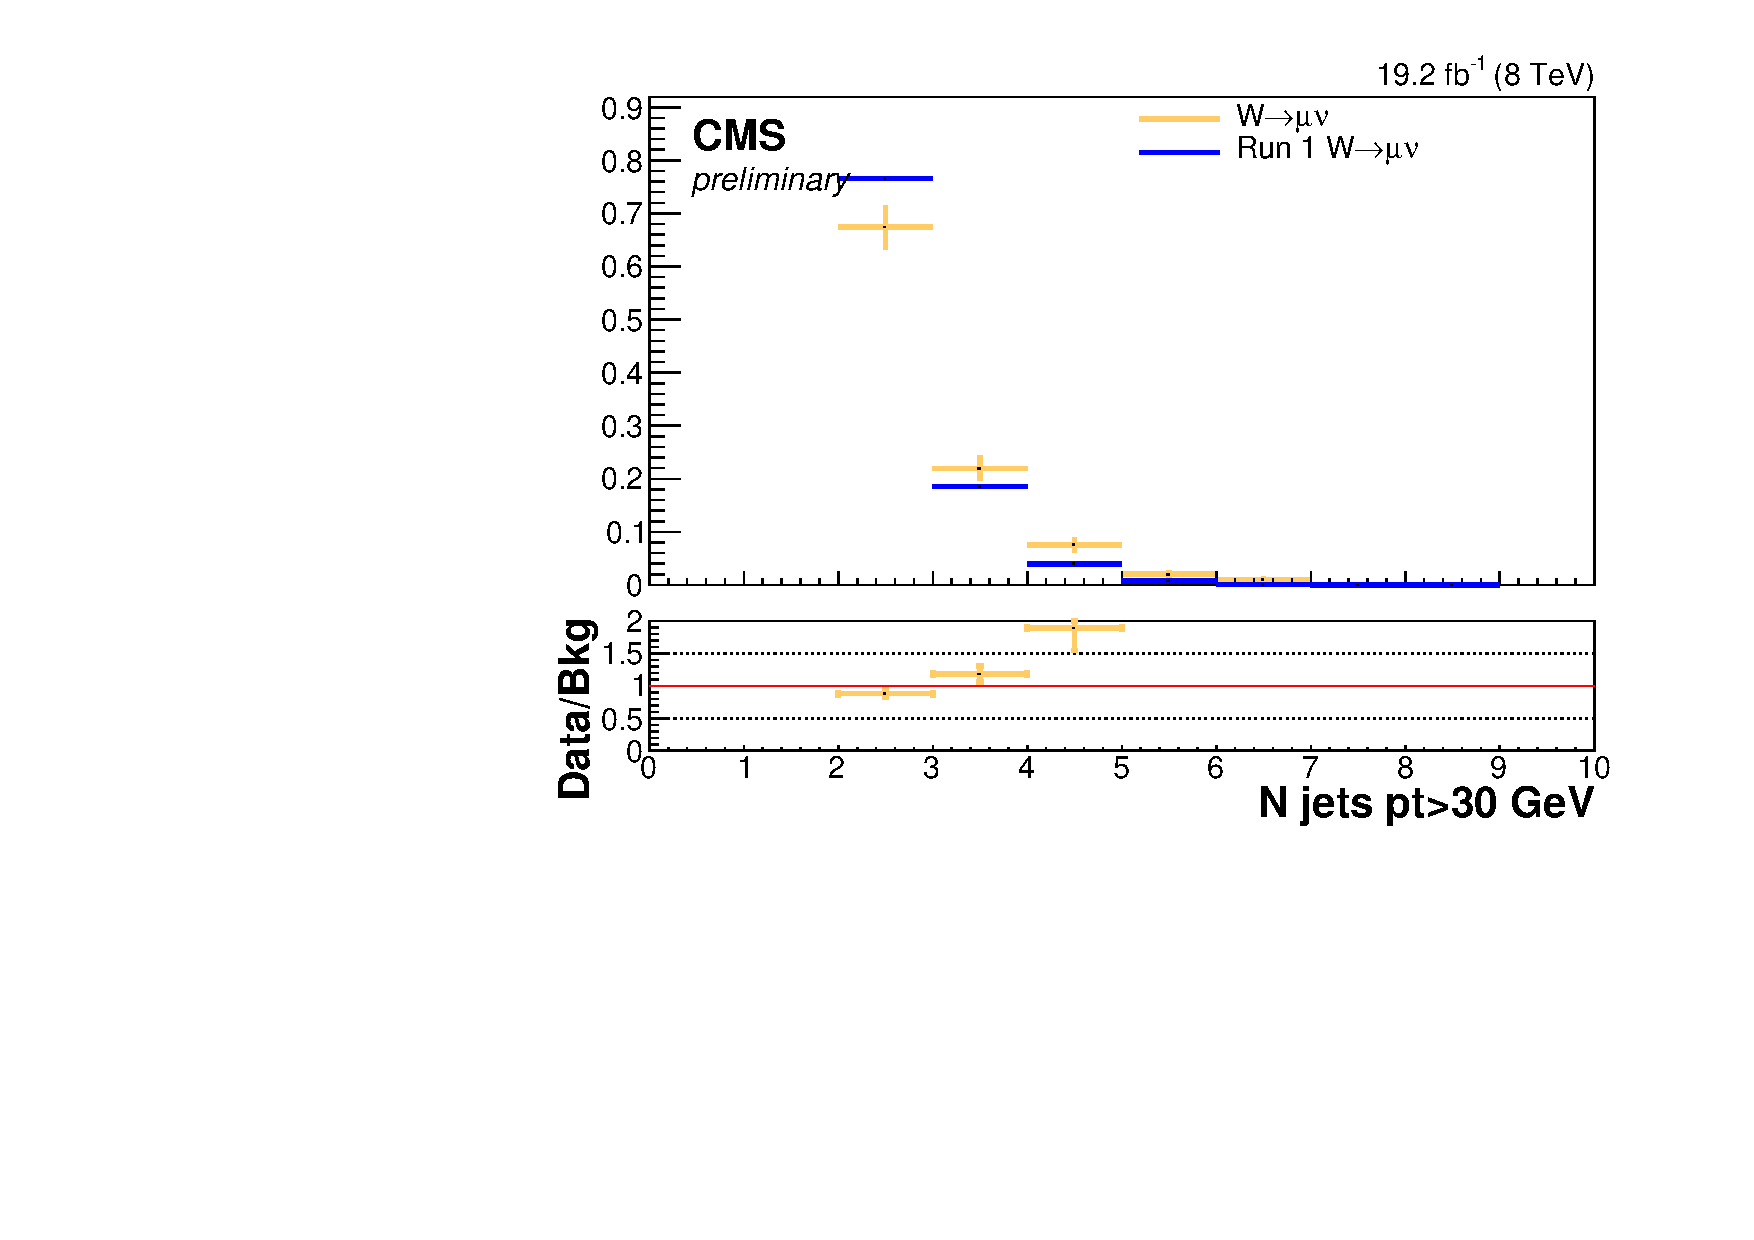
\includegraphics[width=.5\textwidth]{TalkPics/geninfo220615/output_run1comparegen220615/munu_norm_n_jets_30.pdf}
  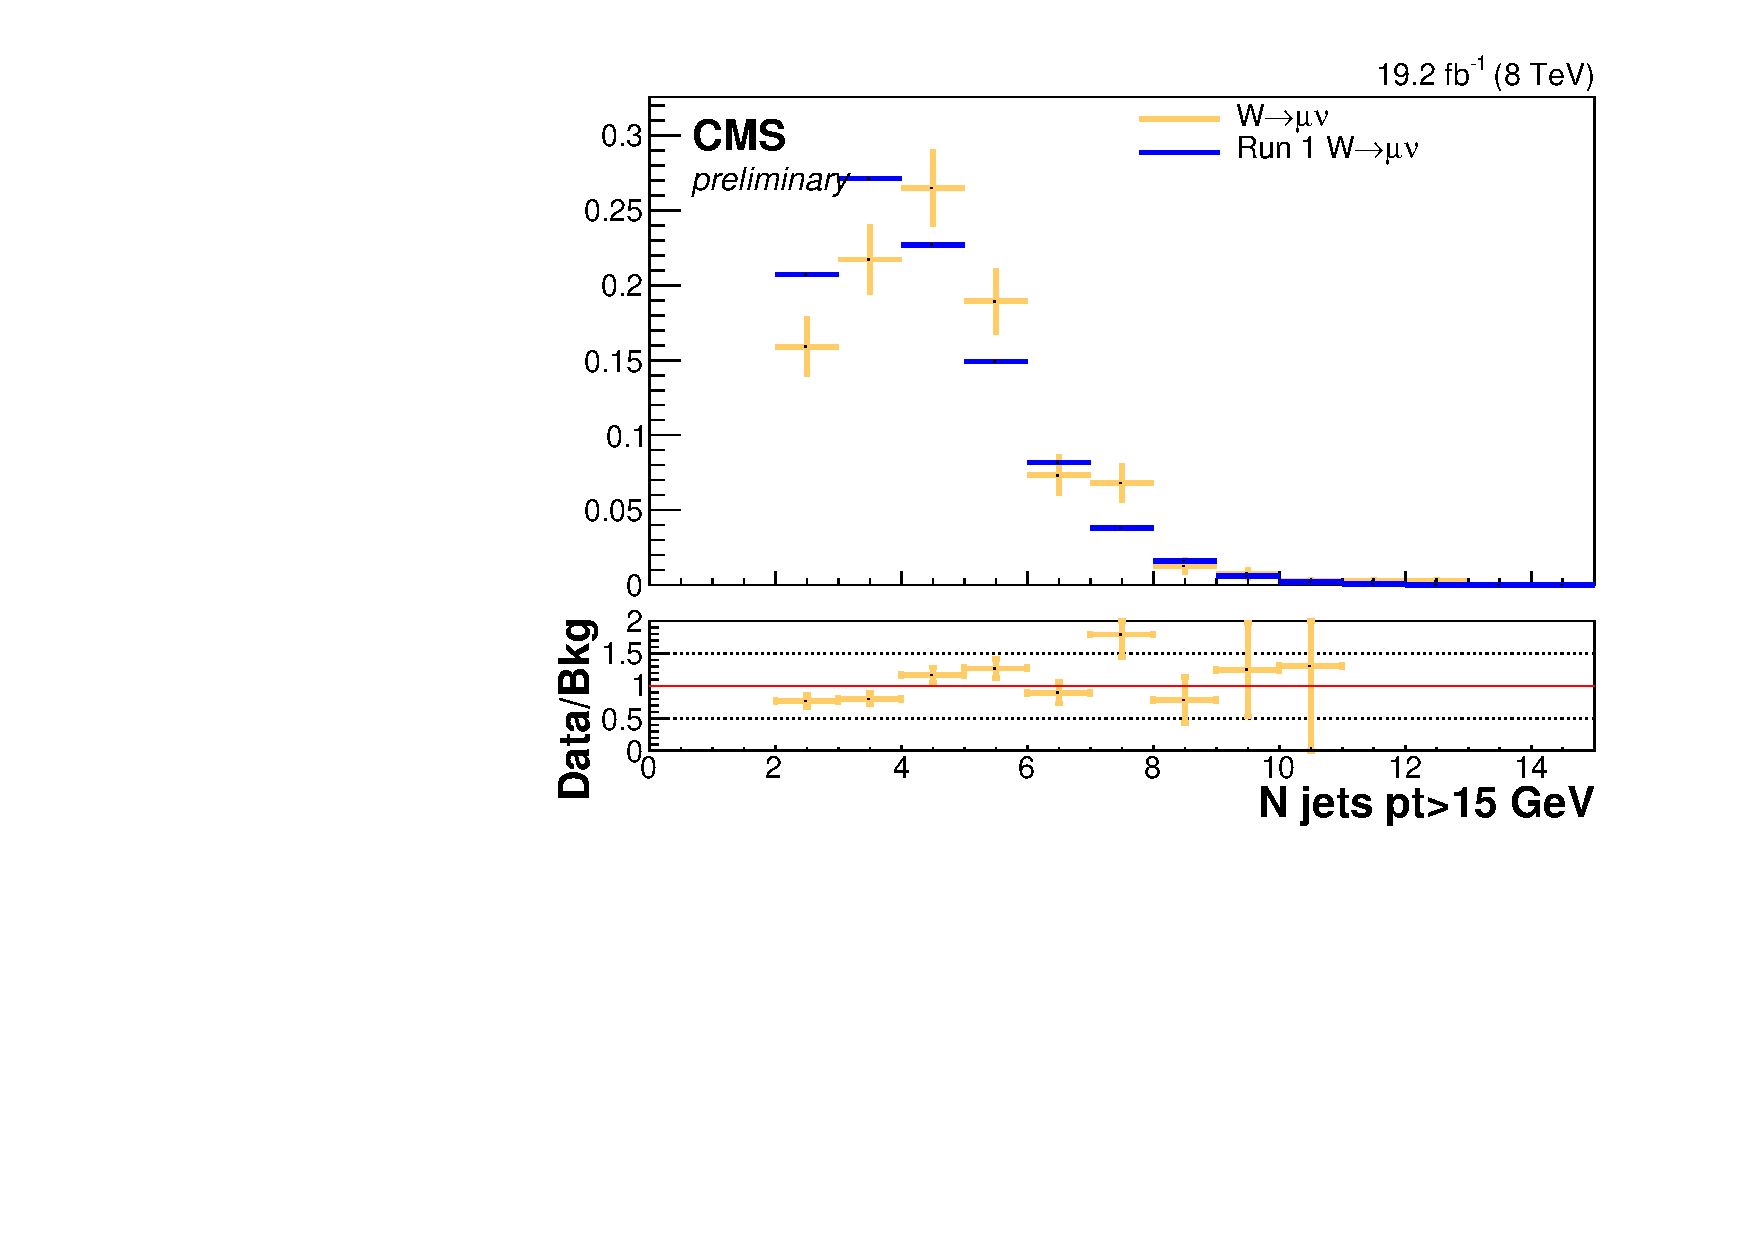
\includegraphics[width=.5\textwidth]{TalkPics/geninfo220615/output_run1comparegen220615/munu_norm_n_jets_15.pdf}
\end{frame}

\begin{frame}
  \begin{block}{}
    \begin{itemize}
    \item Angular variables look more similar after like for like met sig cut
    \item Difference in Mjj and jet pt distributions at low values is interesting
    \item[-] Check gen information
    \item Plotting code issue necessitated restructuring of code
    \end{itemize}
  \end{block}
\end{frame}

\begin{frame}
  \frametitle{W munu Comparison: gen information}
  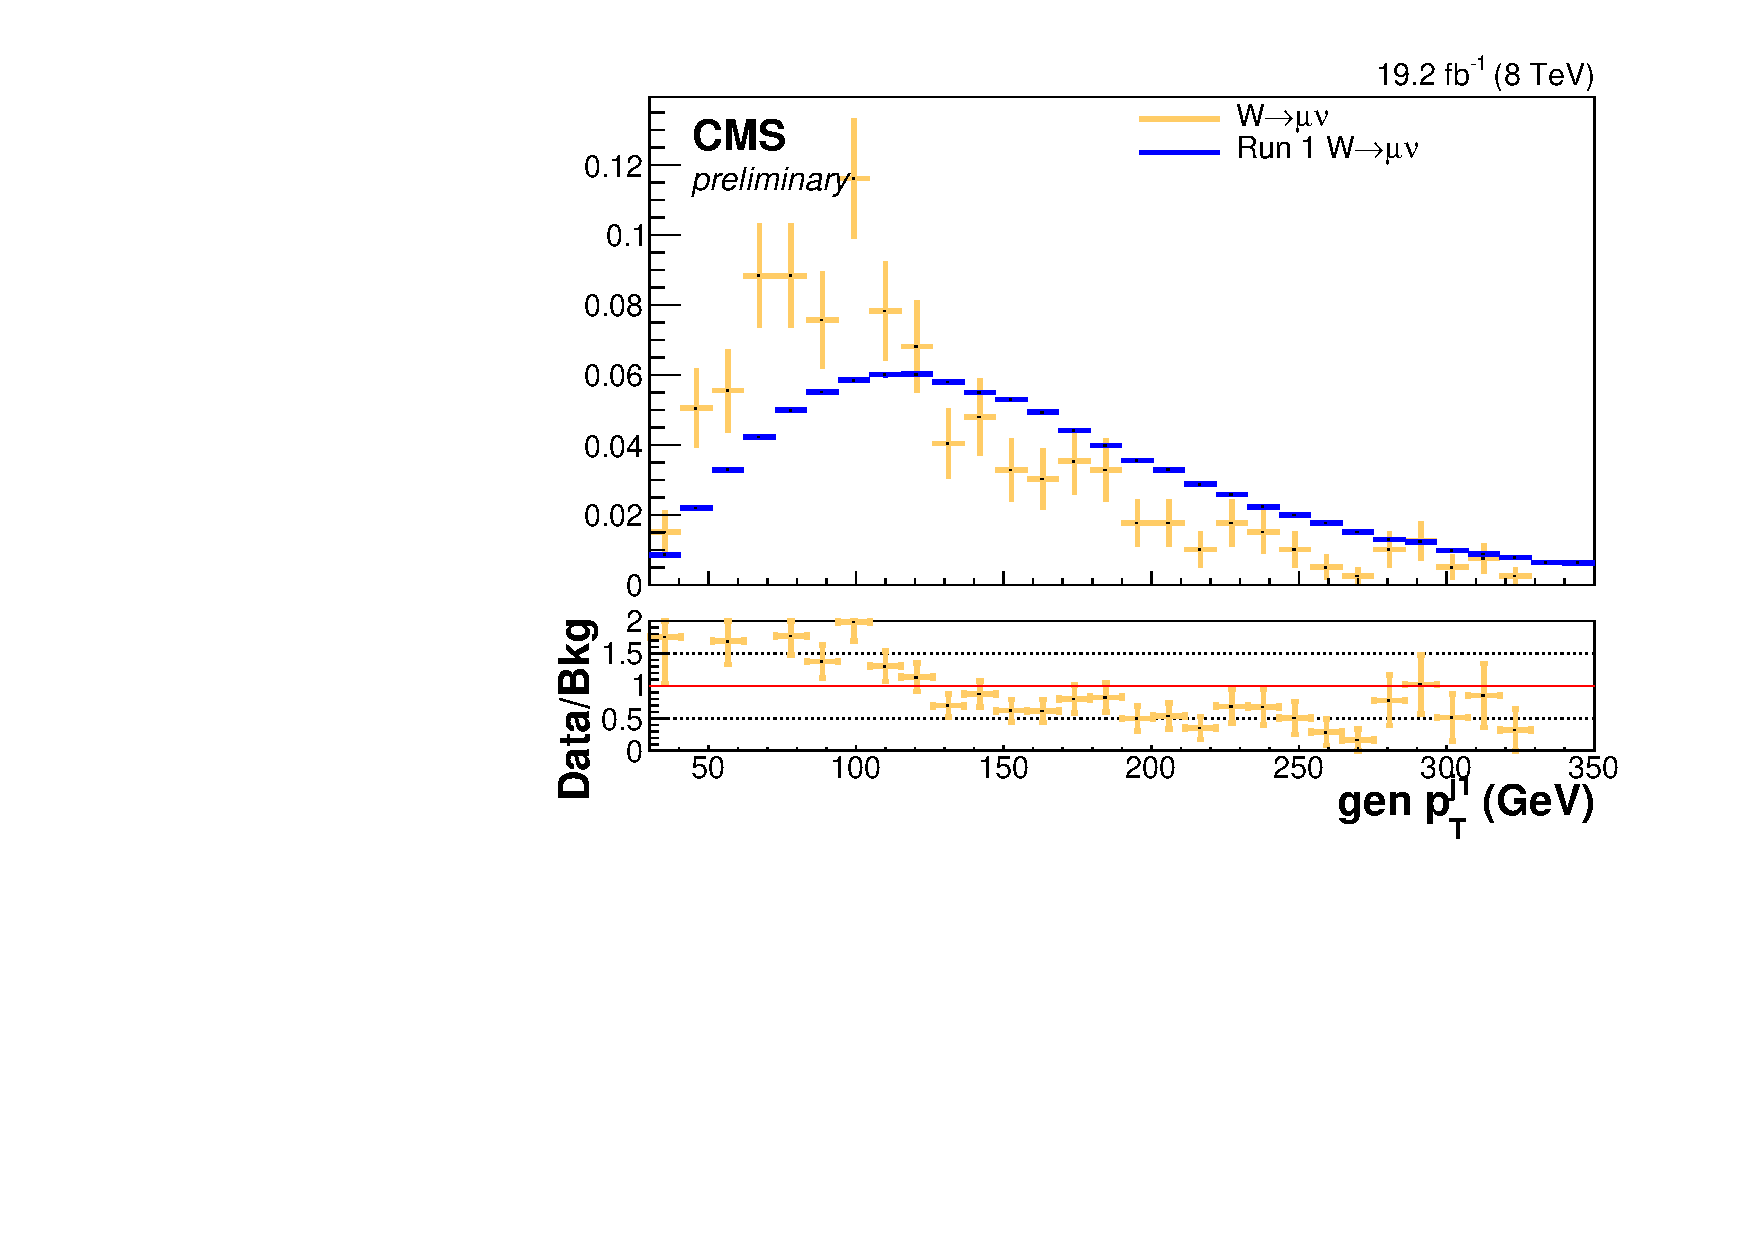
\includegraphics[width=.5\textwidth]{TalkPics/geninfo220615/output_run1comparegen220615/munu_norm_genjet1_pt.pdf}
  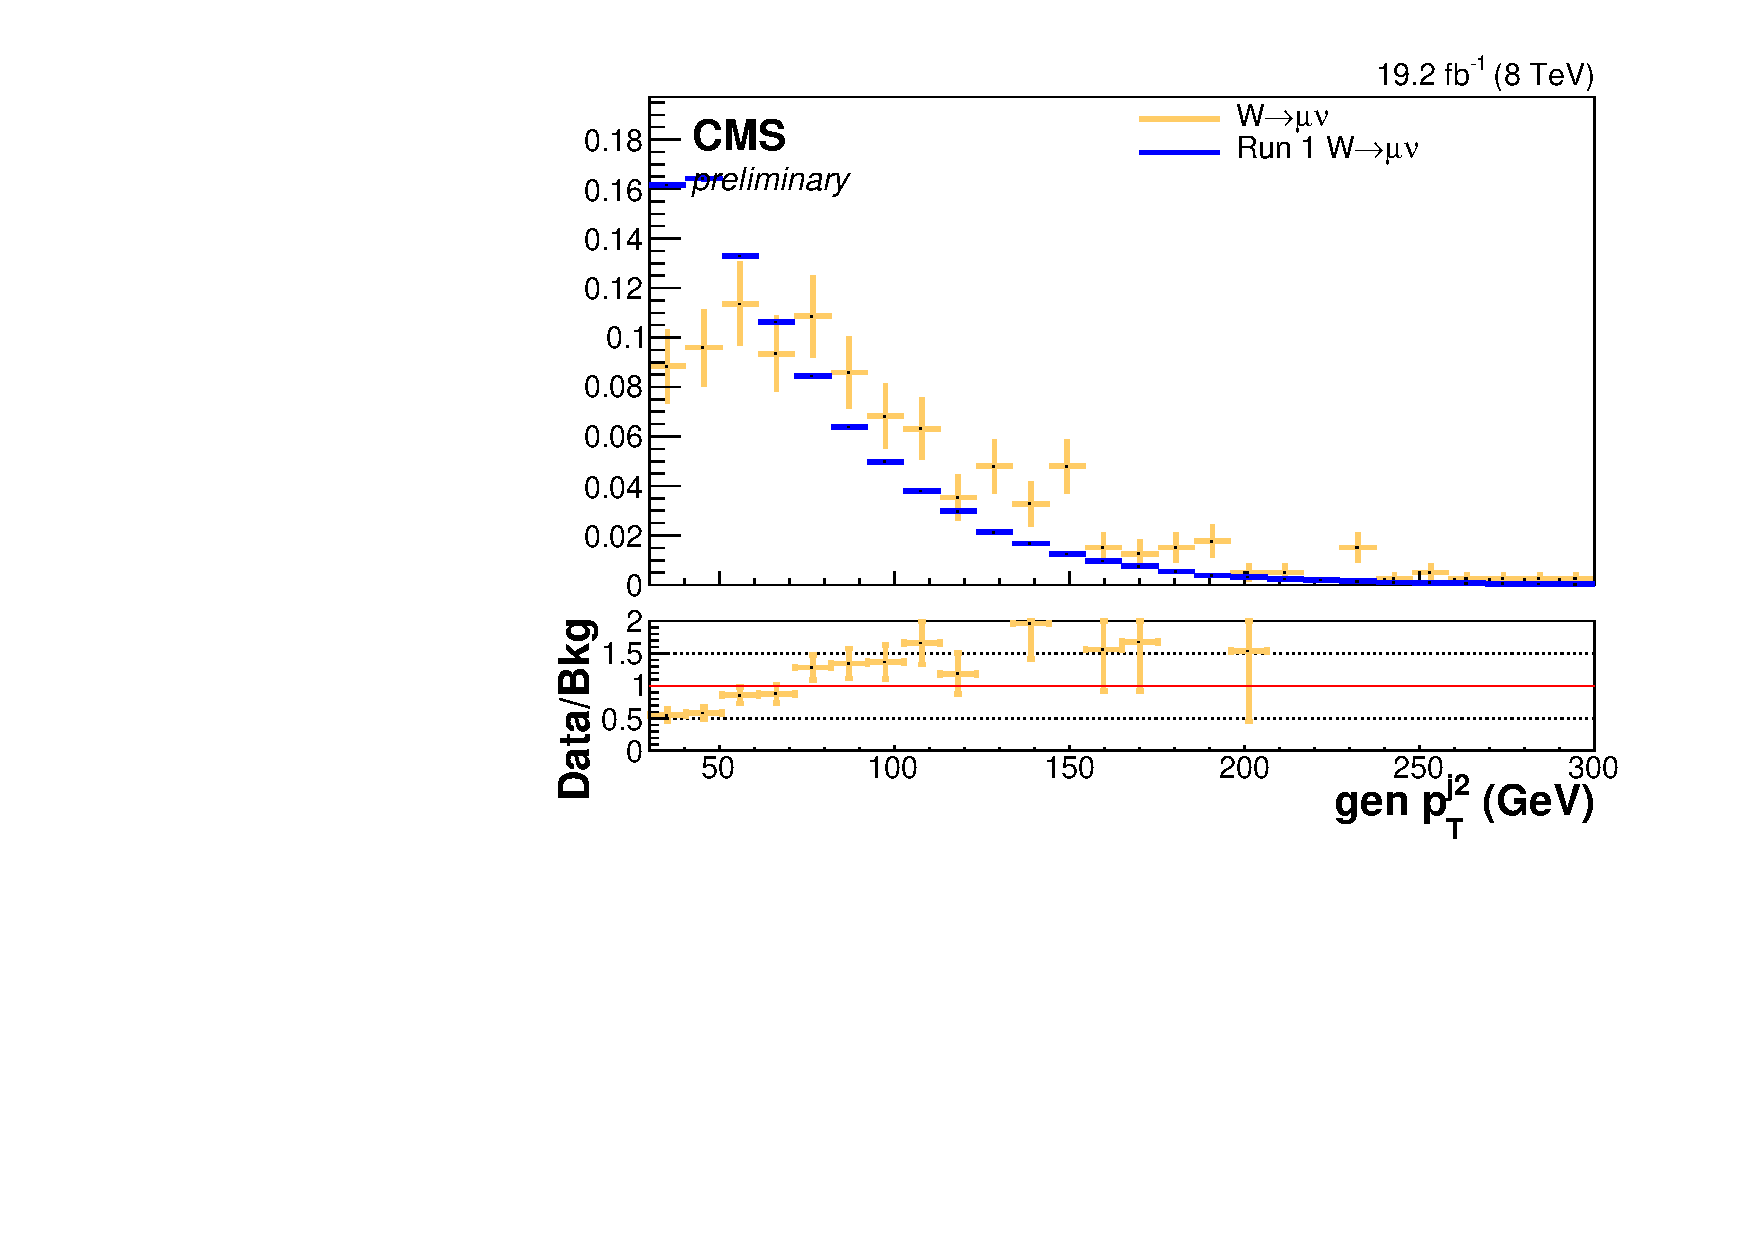
\includegraphics[width=.5\textwidth]{TalkPics/geninfo220615/output_run1comparegen220615/munu_norm_genjet2_pt.pdf}
\end{frame}

\begin{frame}
  \frametitle{W munu Comparison: gen information}
  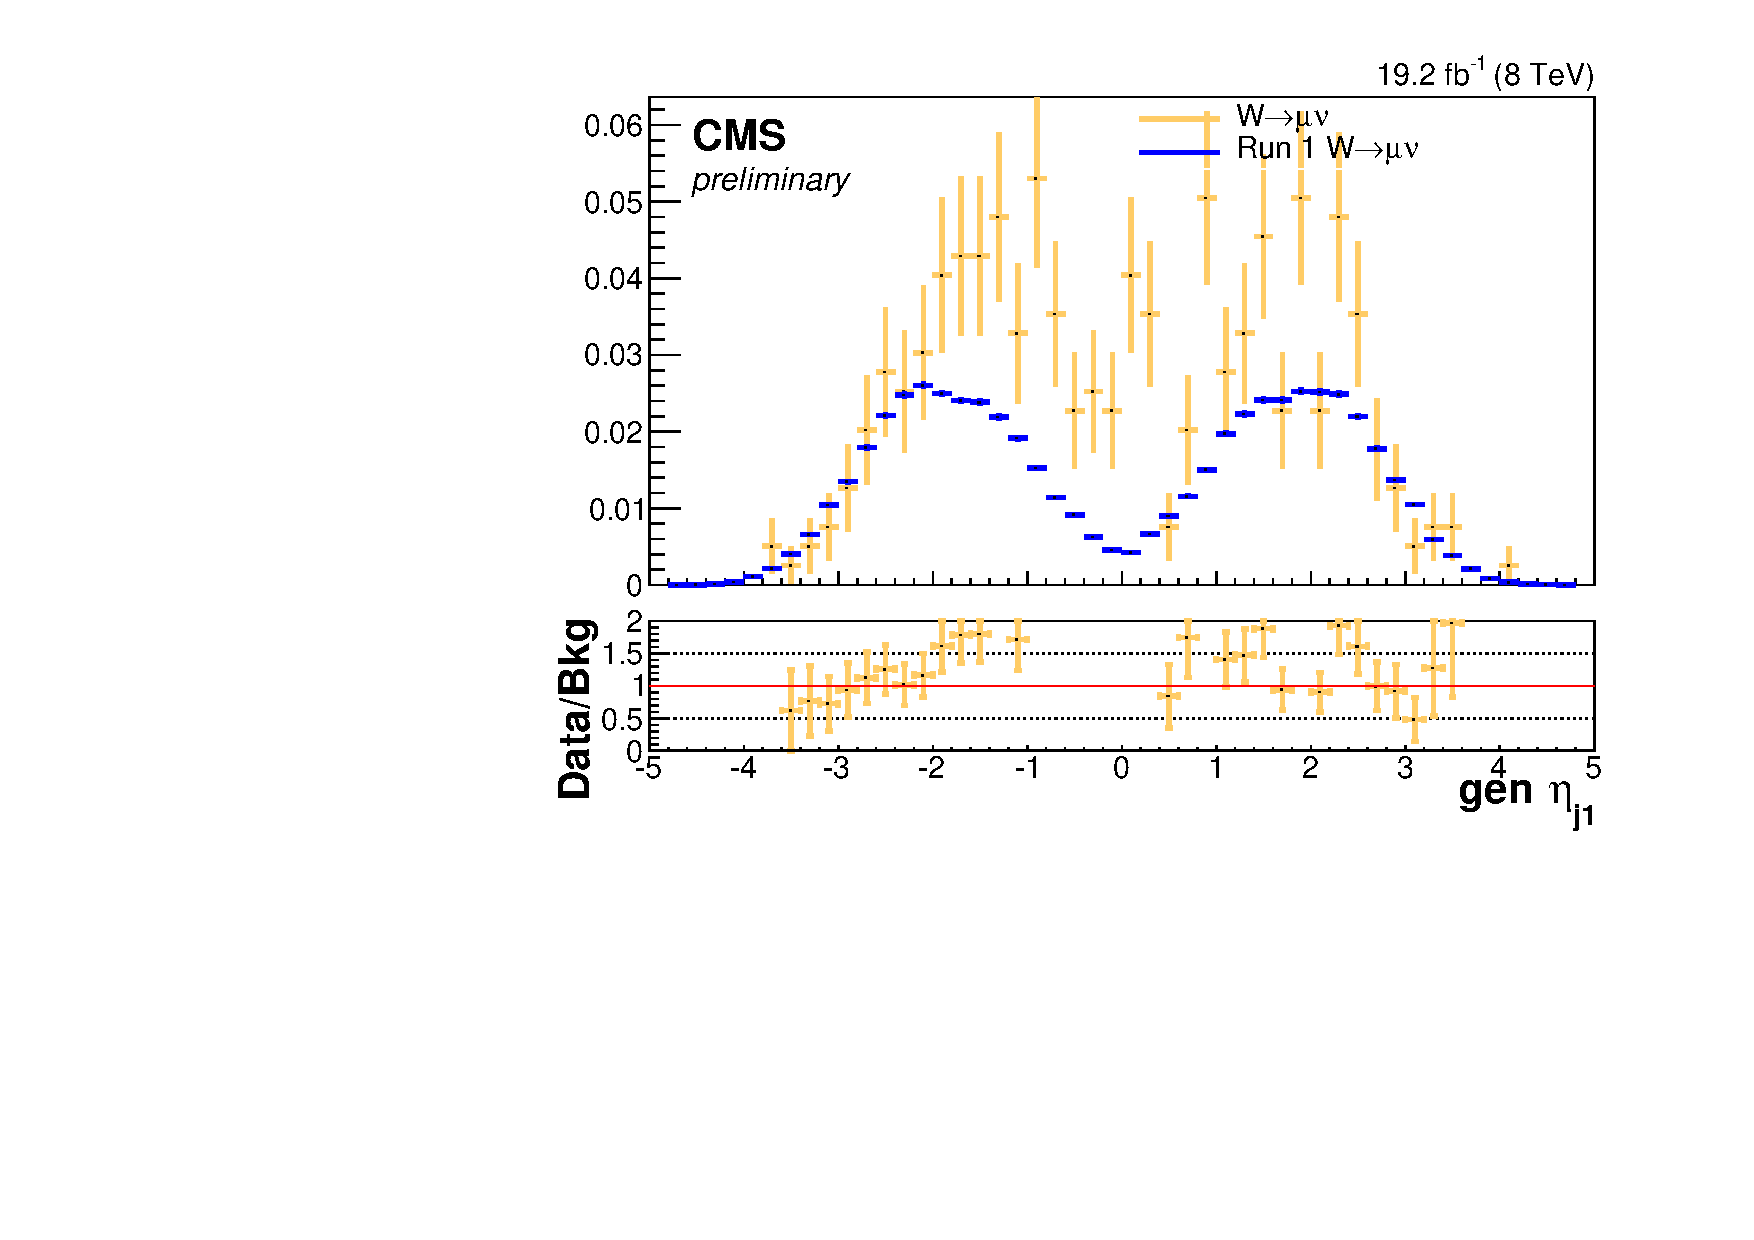
\includegraphics[width=.5\textwidth]{TalkPics/geninfo220615/output_run1comparegen220615/munu_norm_genjet1_eta.pdf}
  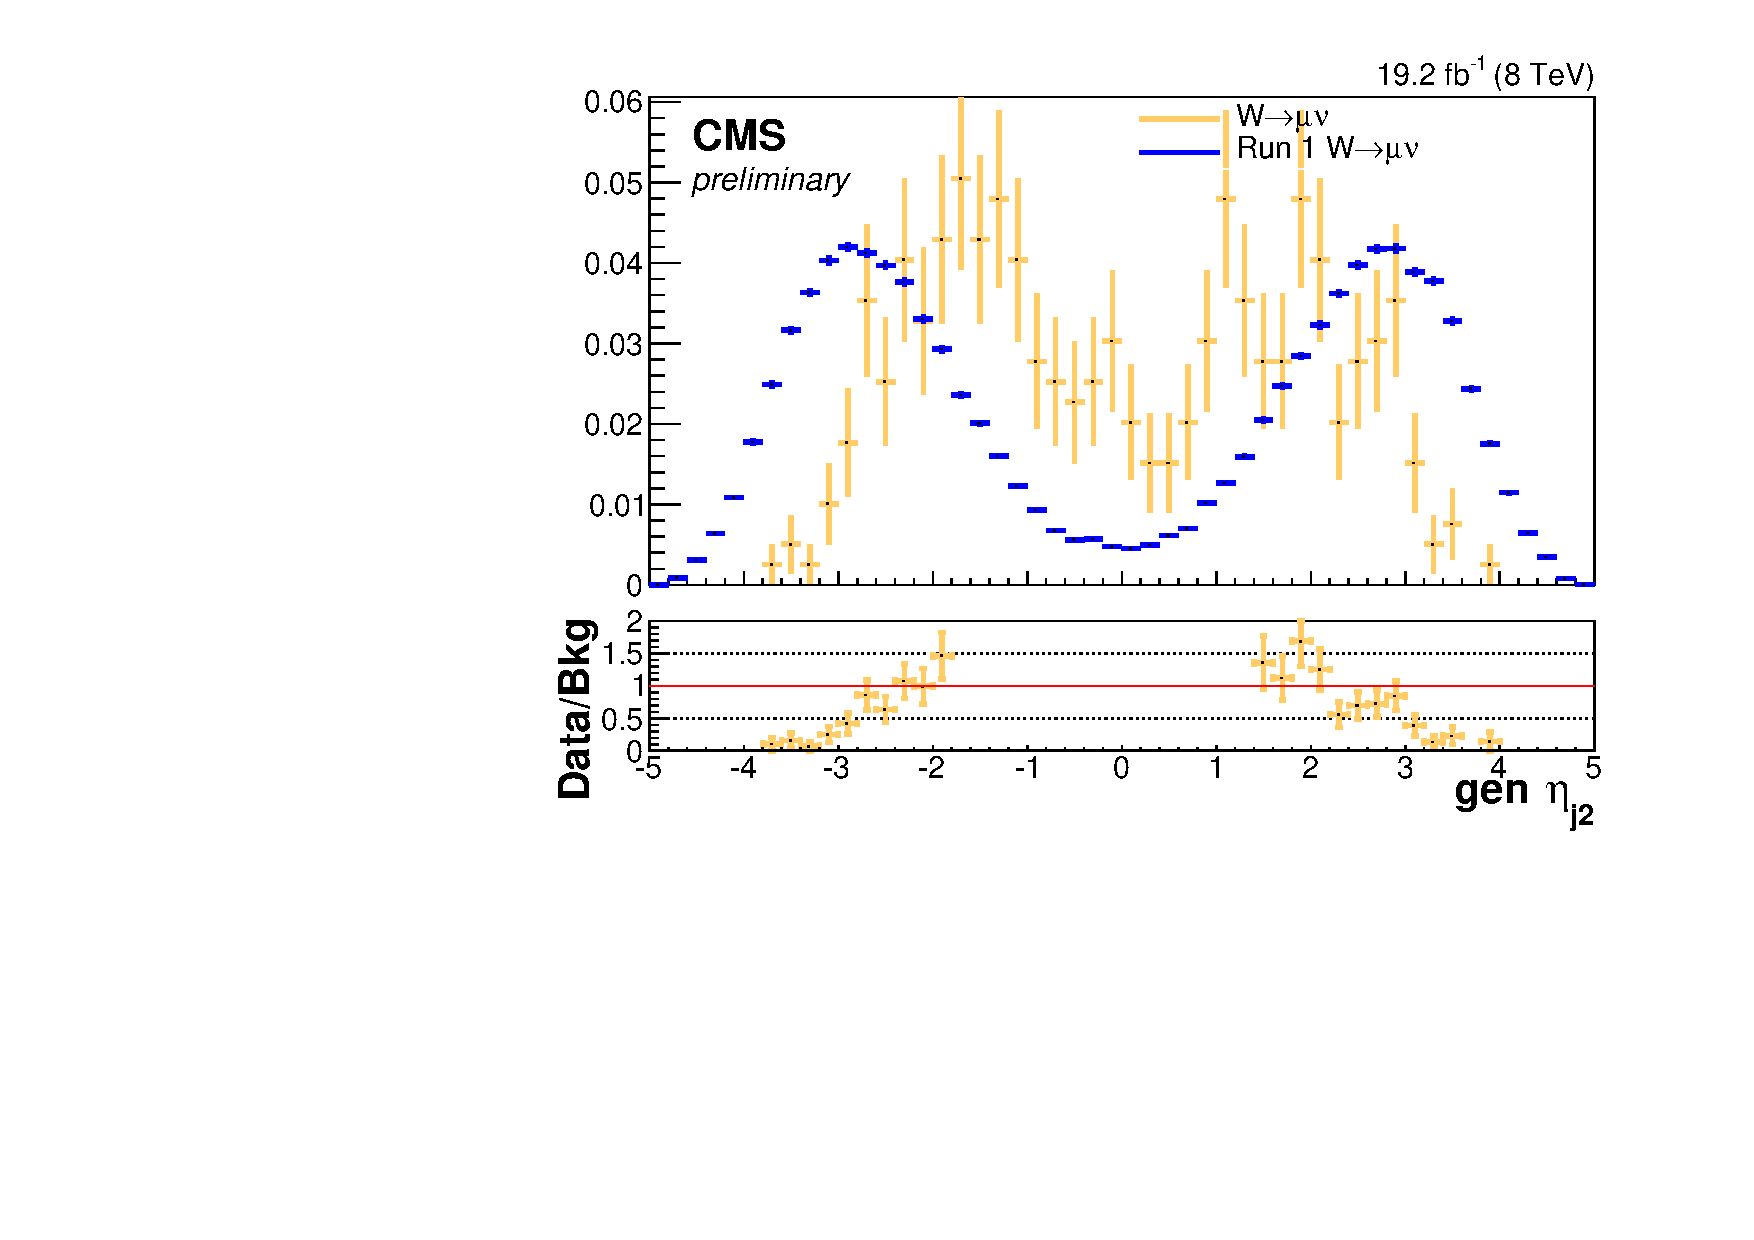
\includegraphics[width=.5\textwidth]{TalkPics/geninfo220615/output_run1comparegen220615/munu_norm_genjet2_eta.pdf}
\end{frame}

\begin{frame}
  \frametitle{W munu Comparison: gen information}
  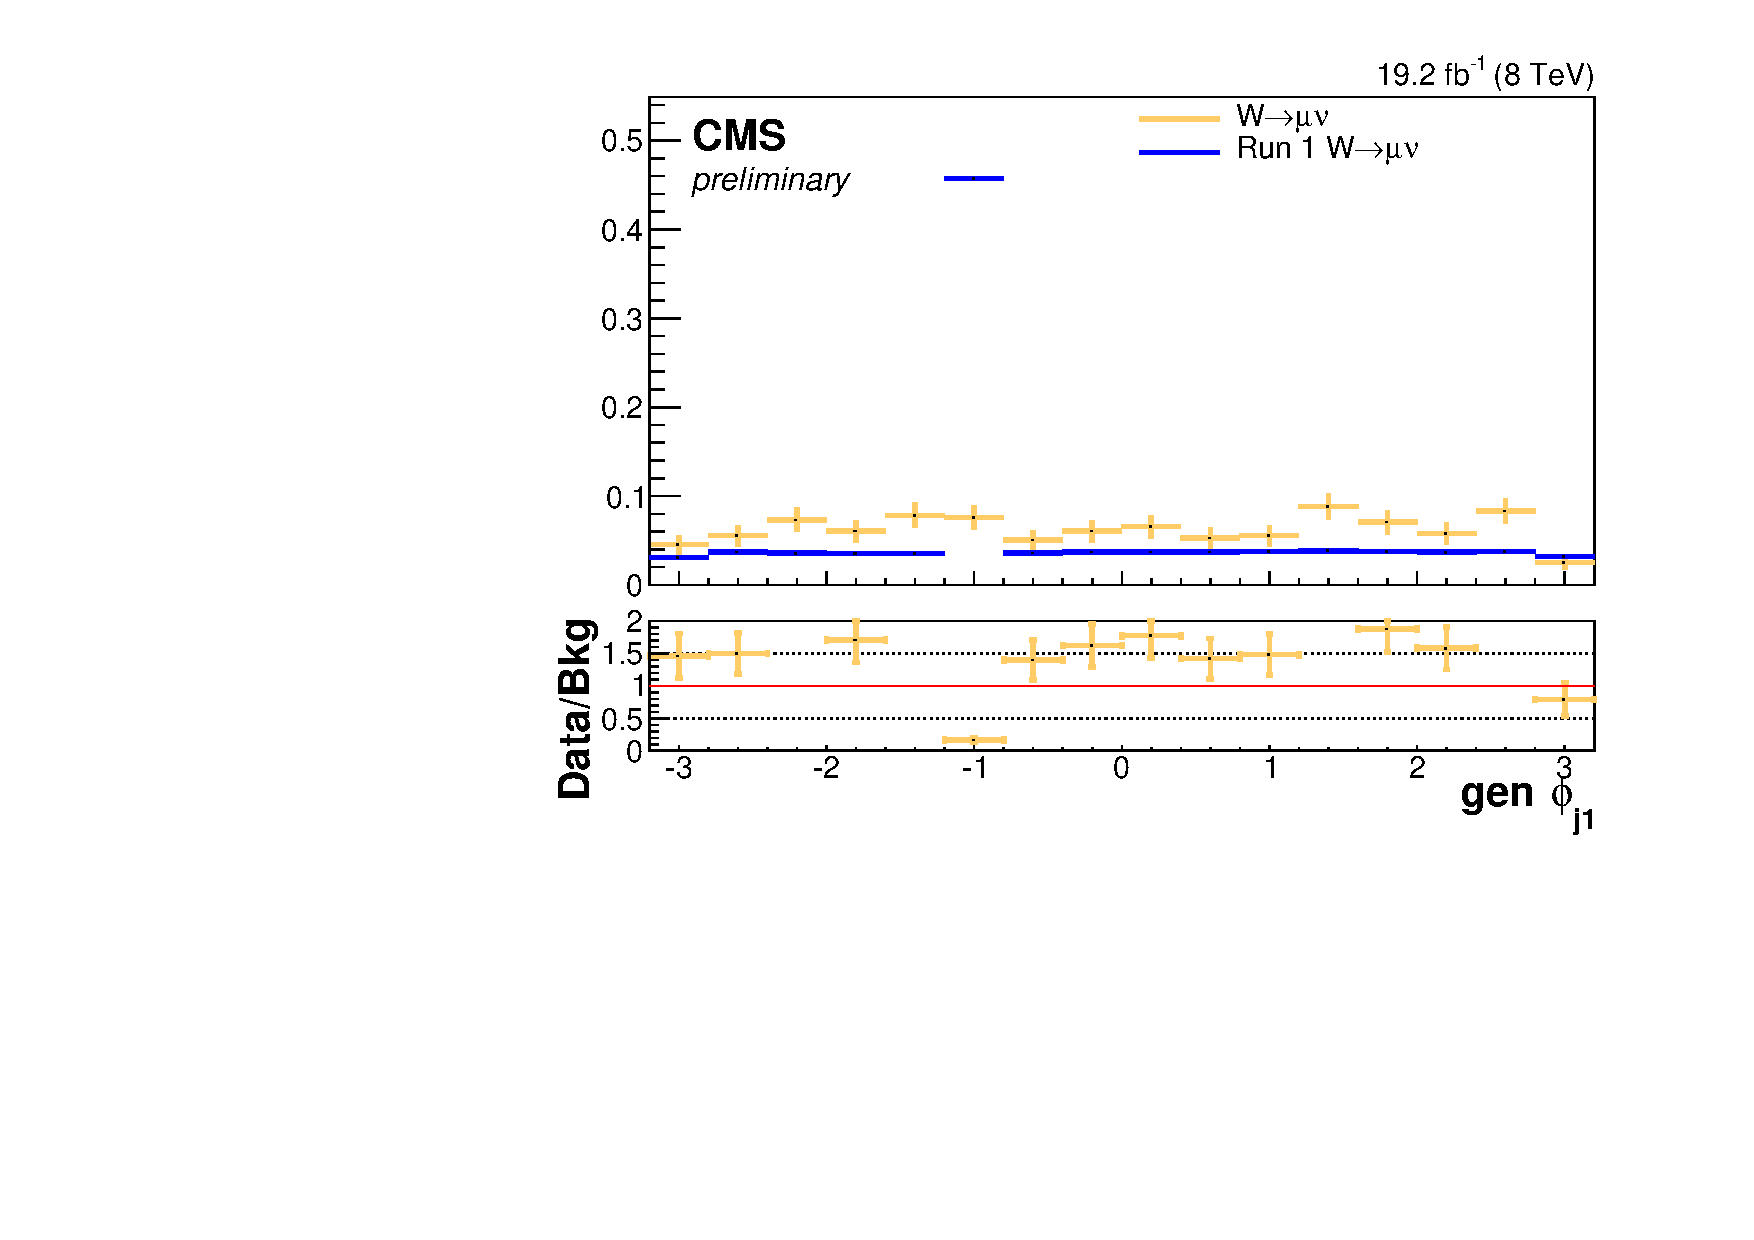
\includegraphics[width=.5\textwidth]{TalkPics/geninfo220615/output_run1comparegen220615/munu_norm_genjet1_phi.pdf}
  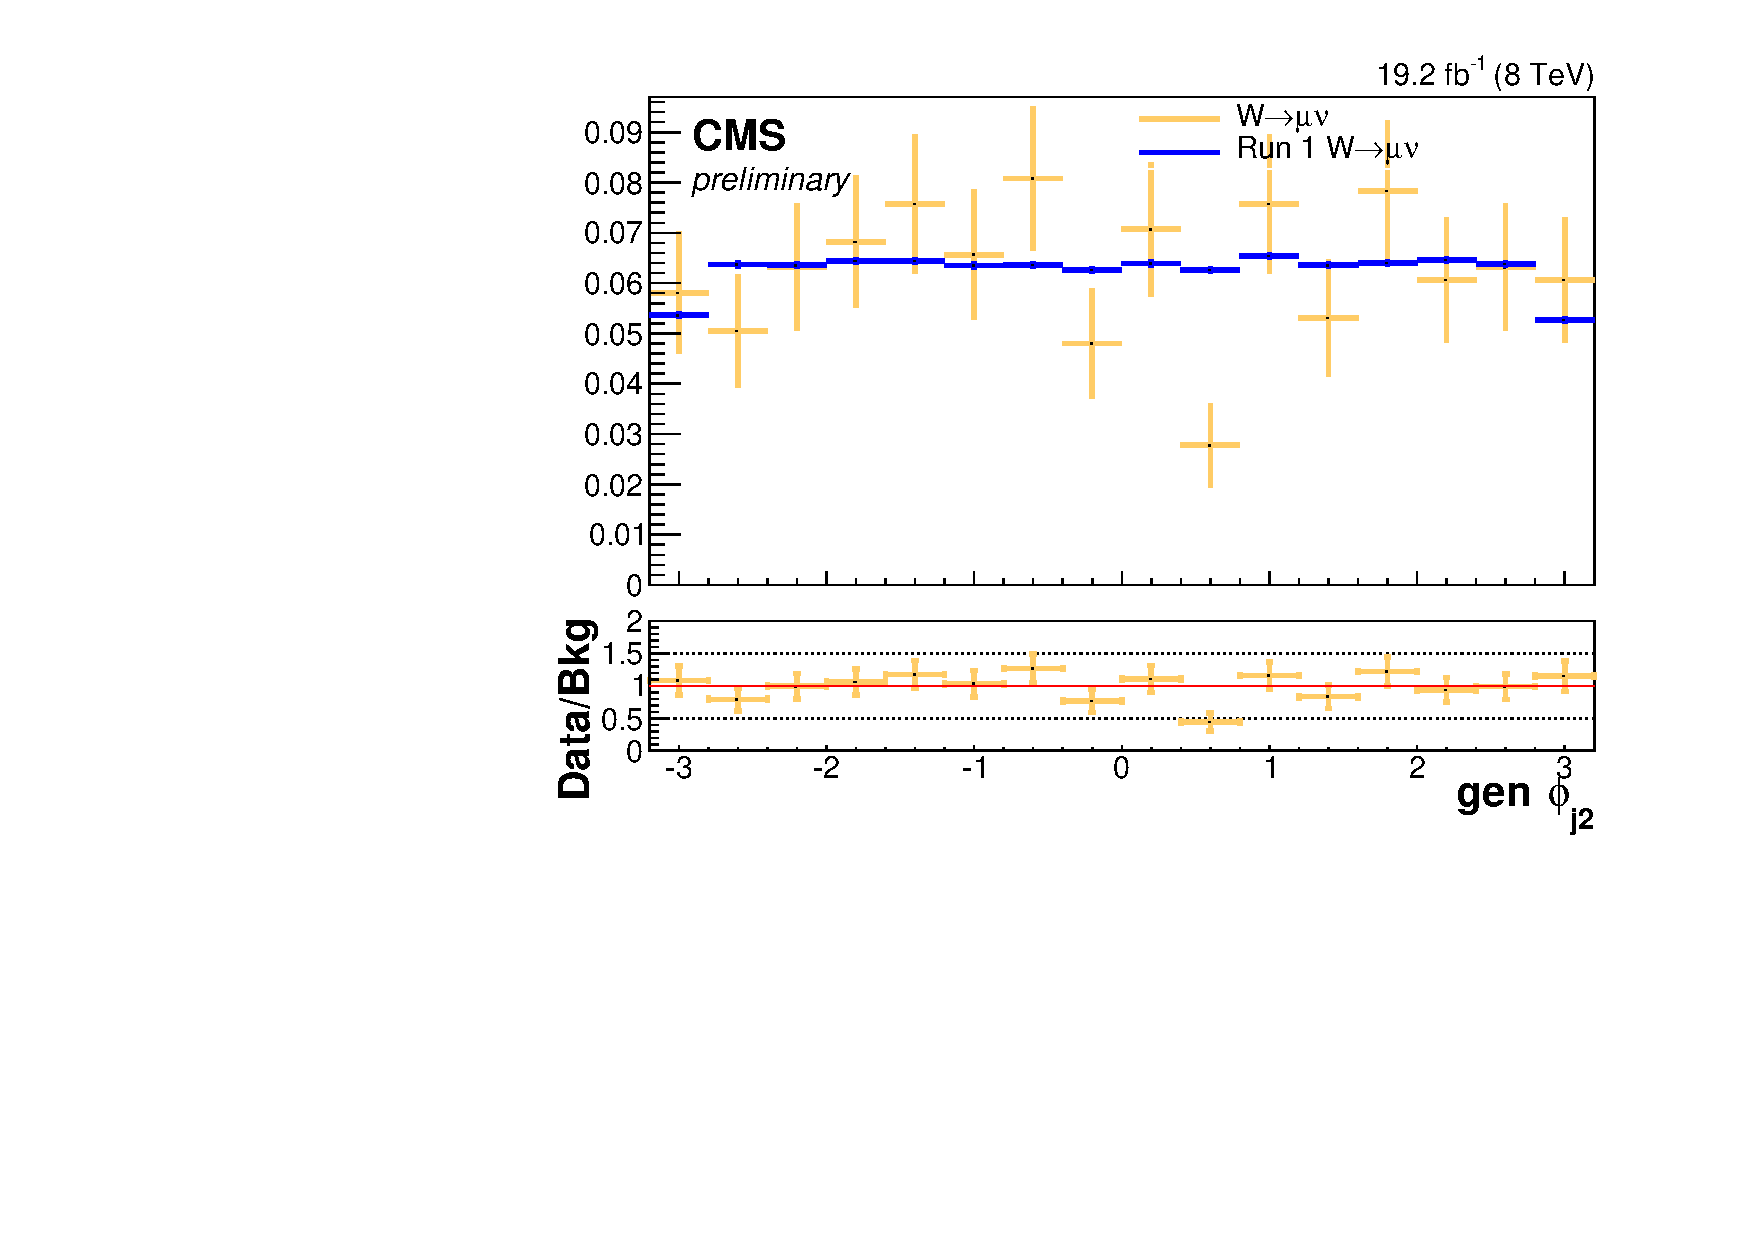
\includegraphics[width=.5\textwidth]{TalkPics/geninfo220615/output_run1comparegen220615/munu_norm_genjet2_phi.pdf}
\end{frame}

\begin{frame}
  \frametitle{W munu Comparison: gen information}
  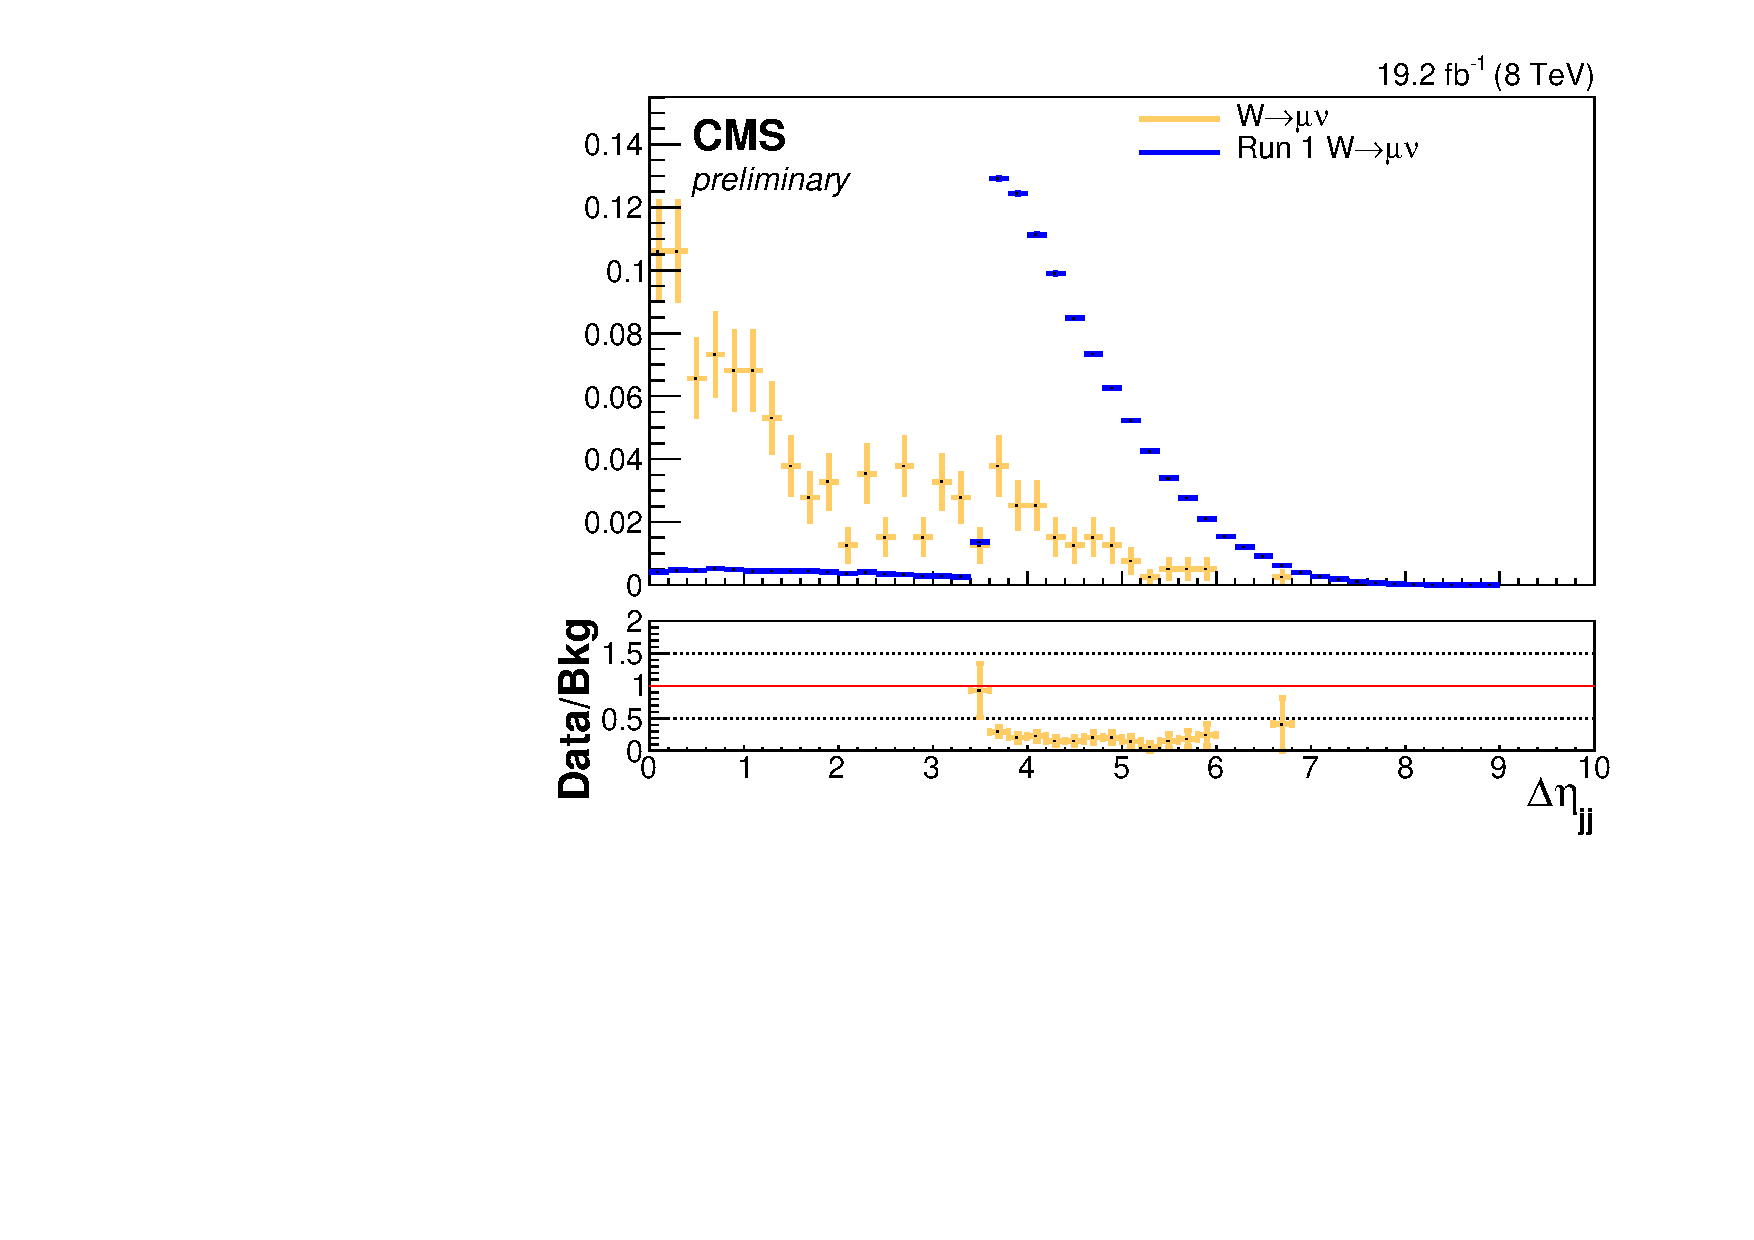
\includegraphics[width=.5\textwidth]{TalkPics/geninfo220615/output_run1comparegen220615/munu_norm_digenjet_deta.pdf}
  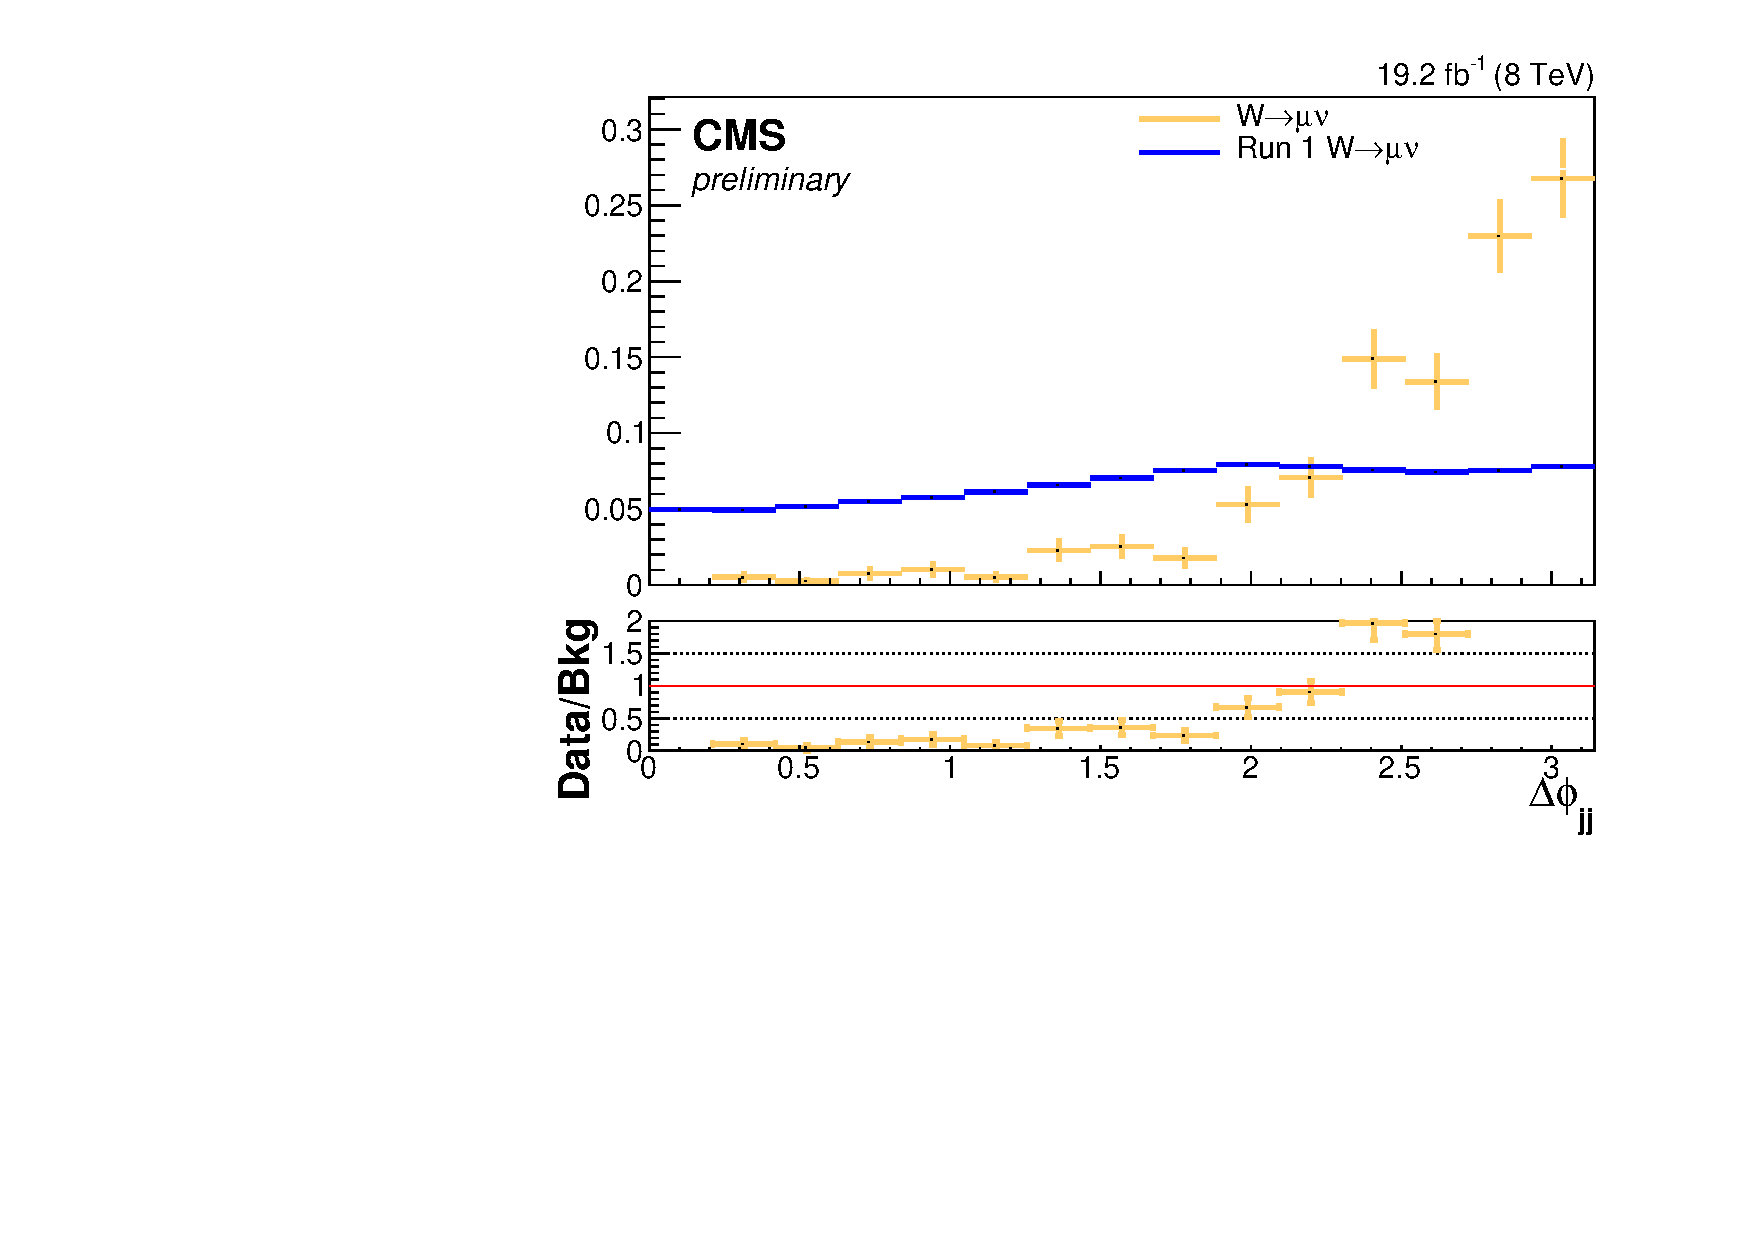
\includegraphics[width=.5\textwidth]{TalkPics/geninfo220615/output_run1comparegen220615/munu_norm_digenjet_dphi.pdf}
\end{frame}

\begin{frame}
  \frametitle{W munu Comparison: gen information}
  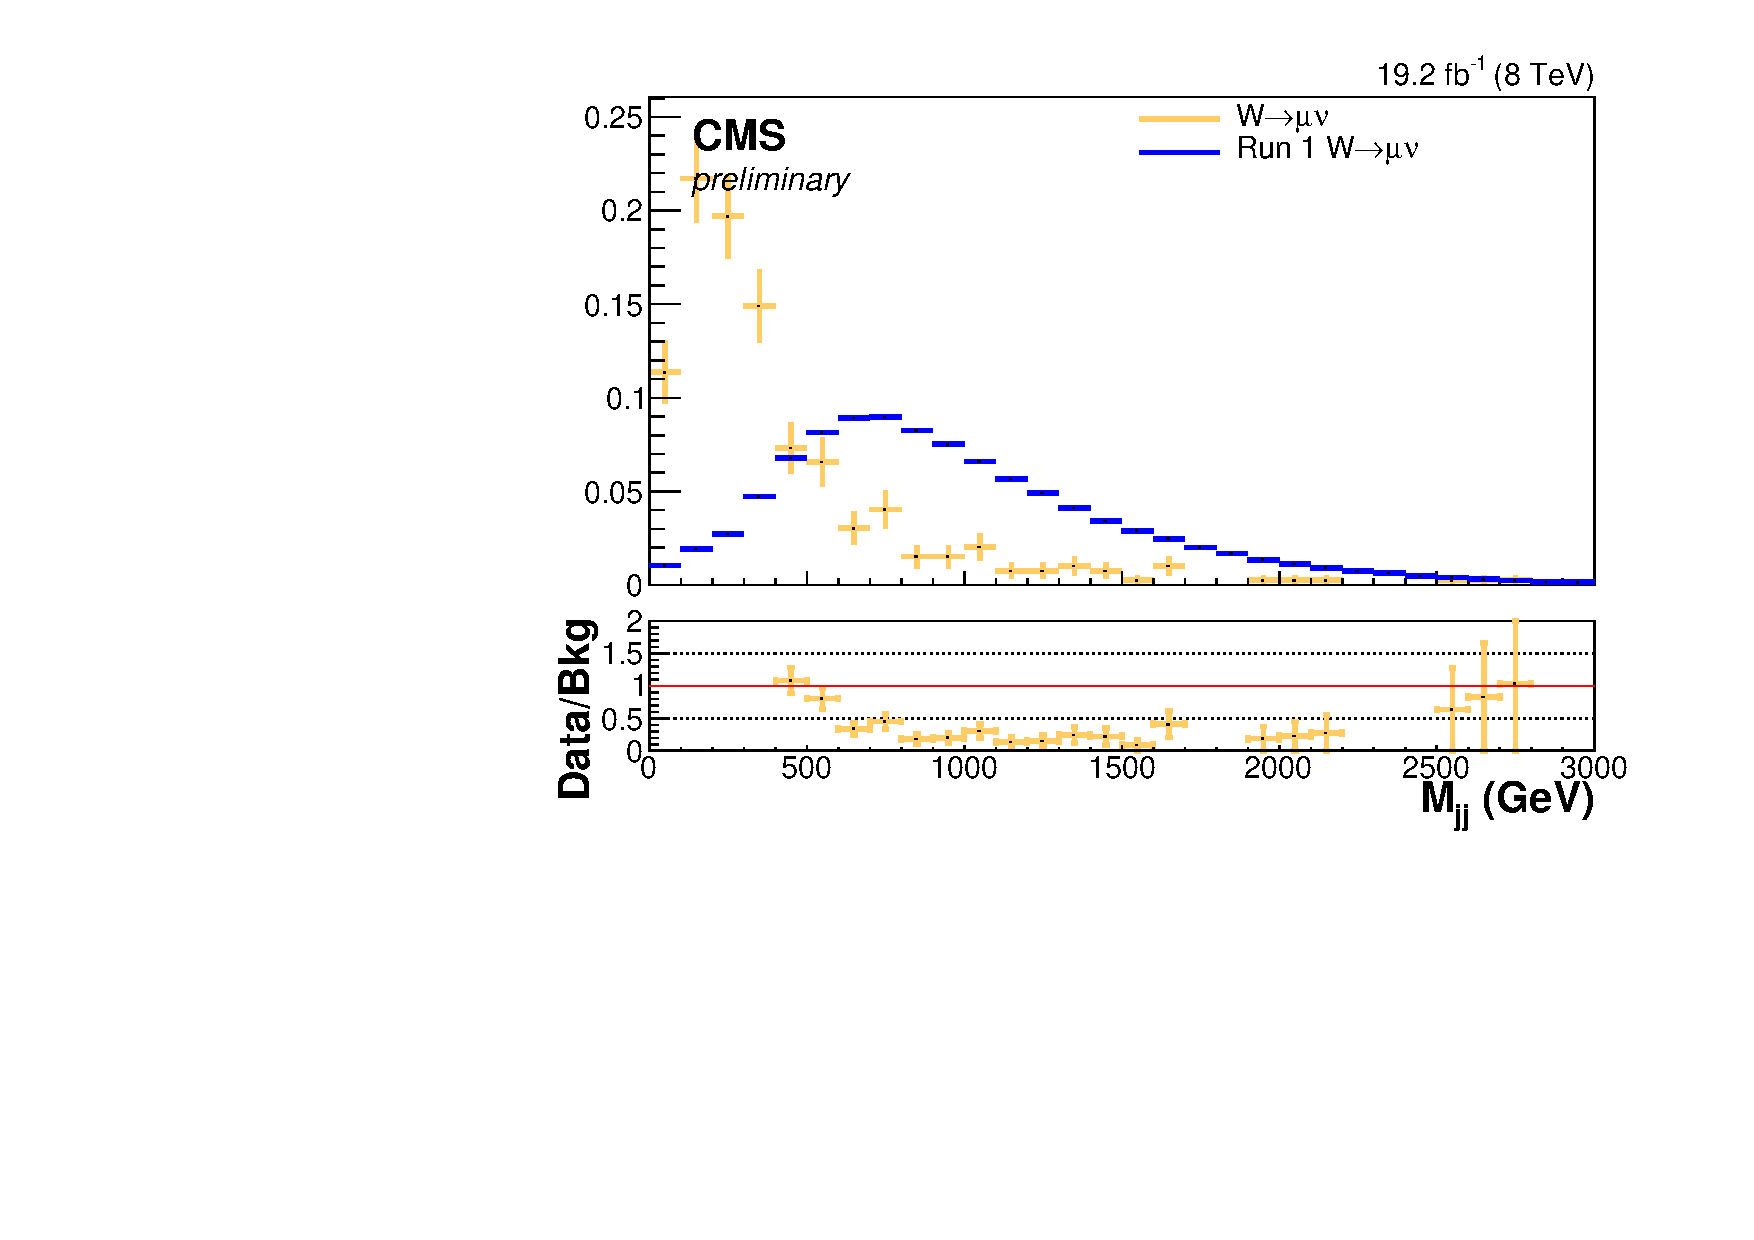
\includegraphics[width=.5\textwidth]{TalkPics/geninfo220615/output_run1comparegen220615/munu_norm_digenjet_M.pdf}
\end{frame}

\begin{frame}
  \label{lastframe}
  \begin{block}{Summary}
    \begin{itemize}
      \item Further investigation of W control plots
      \item Angular variables look very similar after like for like Met sig comparison
      \item Gen variables however very different
      \item[-] Looks like offline leading jets in run 2 are often not the same as at gen level
    \end{itemize}
  \end{block}
\end{frame}

\begin{frame}
  \frametitle{Backup}
\end{frame}

\end{fmffile}
\end{document}
